\chapter{電磁波とマクスウェル作用}

\lectureoverview{まず、源のないマクスウェル方程式を平面波に対して解き、その方程式に偏光、場の幾何学的配置、および速さを決定させる。次に、より深い問いを立てる。すなわち、どのような局所的でローレンツ不変かつゲージ不変な作用が、動的なマクスウェル方程式を生み出すのか。その答えは、電磁場、電荷保存、およびゲージ不変性を一つの構造へと結びつける。}

\section{マクスウェル方程式の二つの族}

平面電磁波から始める。ここで\emph{平面}は幾何学の語であり、飾りのないという意味の\emph{普通の}ではない。直ちに生じる問いは具体的である。そのような波はどのような姿をしているのか、そしてその形はどのようにマクスウェル方程式から従うのか。

波について何かを行う前に、方程式を二つの列に並べておくと有用である。空乏空間ではそれらは
\begin{align}
\nabla\cdot\mathbf B&=0,
&
\dot{\mathbf B}&=\nabla\times\mathbf E,
\label{eq:homogeneous-vector}
\\
\nabla\cdot\mathbf E&=0,
&
\dot{\mathbf E}&=-\,\nabla\times\mathbf B.
\label{eq:dynamical-vector-vacuum}
\end{align}
である。我々はmostly-plus計量
\begin{equation}
\eta_{\mu\nu}=\operatorname{diag}(-1,1,1,1)
\end{equation}
と講義の規約
\begin{equation}
F_{\mu\nu}
=
\partial_\mu A_\nu-\partial_\nu A_\mu,
\qquad
F_{0i}=E_i,
\qquad
F_{ij}=\epsilon_{ijk}B_k.
\label{eq:course-f-convention}
\end{equation}
を用いる。すると同じ二つの族は
\begin{align}
\partial_\mu F_{\nu\sigma}
+\partial_\nu F_{\sigma\mu}
+\partial_\sigma F_{\mu\nu}
&=0,
\label{eq:bianchi-l9}
\\
\partial_\mu F^{\mu\nu}
&=0.
\label{eq:vacuum-maxwell-covariant}
\end{align}
と書ける。

\begin{figure}[H]
\centering
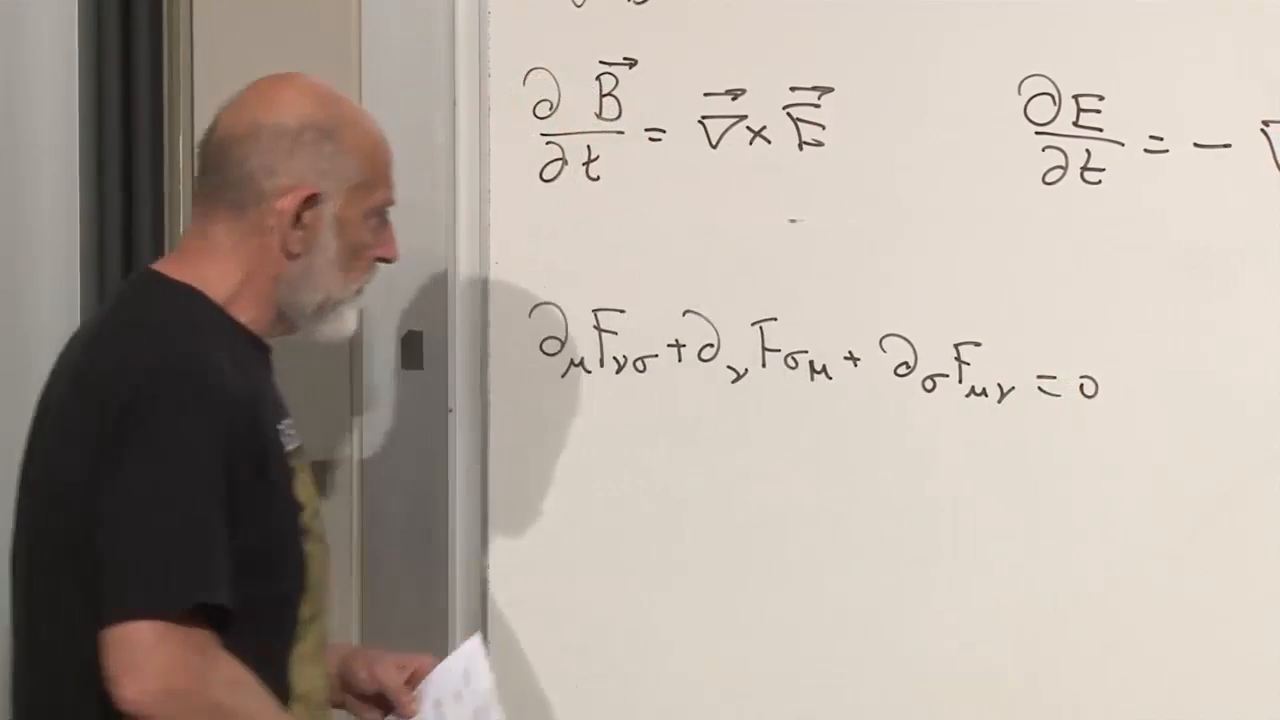
\includegraphics[width=\linewidth]{lecture_09_figure_01.png}
\caption{真空におけるマクスウェル方程式の二つの族とその共変形。巡回方程式は恒等式であり、縮約された方程式は動的である。}
\par\smallskip
\textit{講義フレーム: 00:03:30.}
\end{figure}

二つの行の区別は重要である。方程式
\eqref{eq:bianchi-l9}はポテンシャル\(A_\mu\)の存在から恒等的に従う。すなわち、すべての項は二階導関数であり、項は対になって相殺する。したがってそれはビアンキ恒等式である。対照的に、方程式
\eqref{eq:vacuum-maxwell-covariant}は運動方程式である。電磁ラグランジアンを変えれば、変わるのはこの族である。

この章で二つの役割を果たす小さな観察が黒板にある。マクスウェル方程式に現れるすべての場は微分されている。この事実は平面波の相対位相を制約し、後にゲージ不変性を自然なものにするであろう。

\section{\texorpdfstring{\(z\)}{z}軸に沿った平面波}

波が\(z\)軸に沿って伝播するように座標を選ぶ。これは一般性を失わせない。別の方向の波は軸を回転させることによってこの形に持ち込める。\(k\)をその波数、
\begin{equation}
\lambda=\frac{2\pi}{k},
\end{equation}
とし、\(\omega\)をその振動数とする。運動方程式を課す前に、六つの場の成分すべてを共通の位相
\begin{equation}
\theta=kz-\omega t:
\end{equation}
\begin{align}
E_x(z,t)&=\epsilon_x\sin\theta,
&
B_x(z,t)&=\beta_x\sin\theta,
\nonumber\\
E_y(z,t)&=\epsilon_y\sin\theta,
&
B_y(z,t)&=\beta_y\sin\theta,
\label{eq:plane-wave-ansatz}\\
E_z(z,t)&=\epsilon_z\sin\theta,
&
B_z(z,t)&=\beta_z\sin\theta.
\nonumber
\end{align}
で書く。六つのギリシャ文字は定数振幅である。

\begin{figure}[H]
\centering
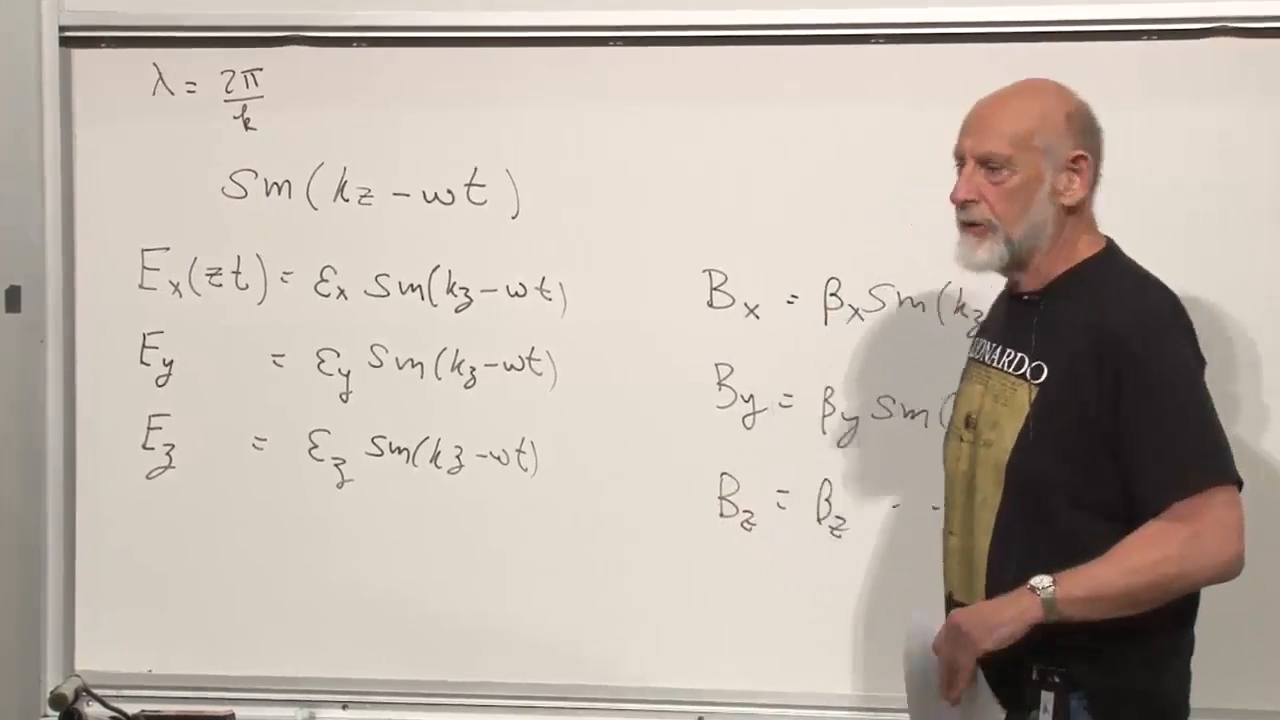
\includegraphics[width=\linewidth]{lecture_09_figure_02.png}
\caption{マクスウェル方程式が禁じられた振幅を取り除く前の、六成分平面波の仮定。}
\par\smallskip
\textit{講義フレーム: 00:08:45.}
\end{figure}

なぜ\(\mathbf E\)と\(\mathbf B\)に対して同じ正弦的依存性から始めるのか。一方の場が\(\sin\theta\)を伴い、他方の場が\(\cos\theta\)を伴うと仮定しよう。すると、回転方程式の片側の時間微分と反対側の空間微分は異なる三角関数を生み出すであろう。等式はすべての\(z\)と\(t\)に対して成り立つことはできない。共通の定数位相は許されるが、\(z\)の原点を平行移動すればそれは除かれる。したがってこの仮定は追加の動的法則ではなく、微分方程式が要求する位相関係の最も単純な代表である。

まだどのマクスウェル方程式も使われていない。我々はただ方向、波長、そして都合のよい位相原点を選んだだけである。ここで方程式がどの振幅が生き残るかを決めるであろう。

\subsection{発散の制約}

場は\(z\)と\(t\)のみに依存するので、
\begin{equation}
\nabla\cdot\mathbf E
=
\partial_xE_x+\partial_yE_y+\partial_zE_z
=
\partial_zE_z.
\end{equation}
である。空乏空間ではこれはすべての位相に対して消えなければならないから、
\begin{equation}
\epsilon_z=0.
\label{eq:epsilon-z-zero}
\end{equation}
である。磁場についても同じ議論から
\begin{equation}
\beta_z=0.
\label{eq:beta-z-zero}
\end{equation}
が得られる。どちらの場も伝播方向に沿った成分を持たない。波は横波である。

横方向の\(xy\)面には回転の自由度が残っている。組\((\epsilon_x,\epsilon_y)\)は通常の二次元ベクトルであるから、横軸を
\begin{equation}
\epsilon_y=0,
\qquad
\epsilon_x\ne0.
\label{eq:polarization-axis}
\end{equation}
となるまで回転させる。これは直線偏光の選択であり、物理に対する制限ではない。

\begin{figure}[H]
\centering
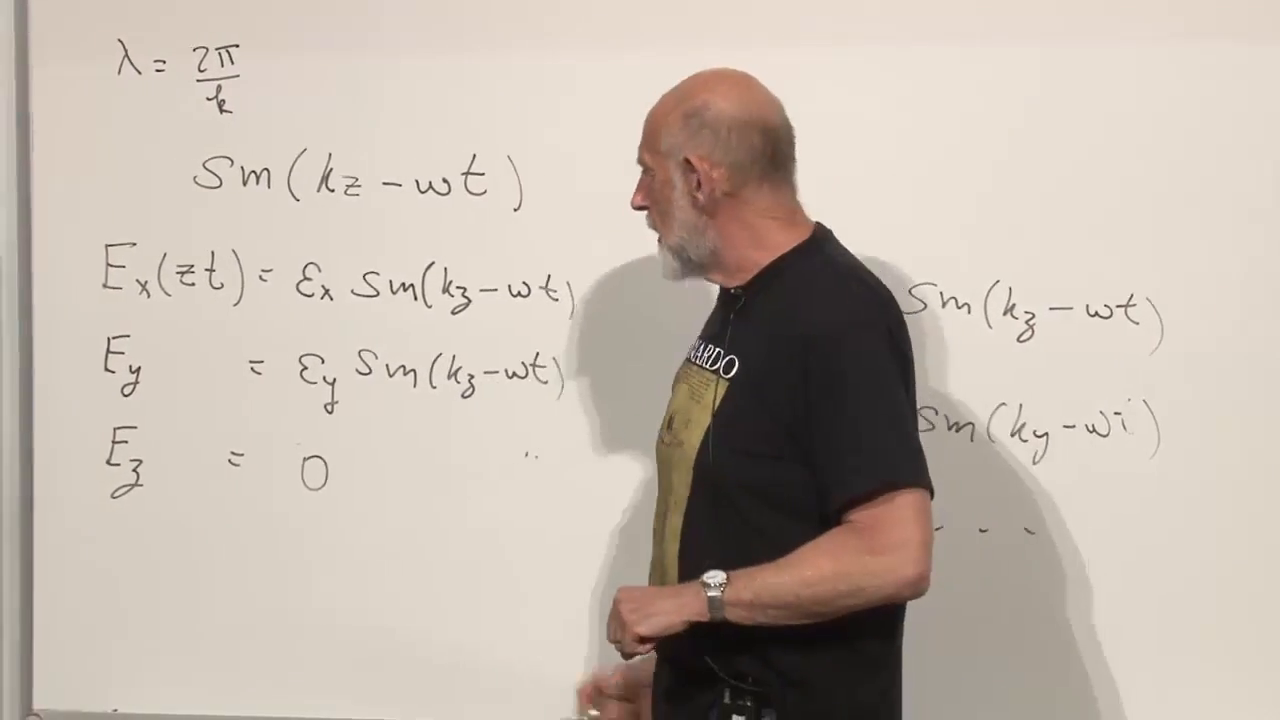
\includegraphics[width=\linewidth]{lecture_09_figure_03.png}
\caption{縦方向の振幅は消え、横方向の電気軸が選ばれた。}
\par\smallskip
\textit{講義フレーム: 00:14:30.}
\end{figure}

\subsection{回転方程式}

\(x\)成分の
\(\dot{\mathbf E}=-\nabla\times\mathbf B\)
を用いる。場は\(z\)のみに依存するので、
\begin{equation}
\dot E_x
=
-\left(\nabla\times\mathbf B\right)_x
=
\partial_zB_y.
\end{equation}
である。仮定を代入すると
\begin{align}
-\omega\epsilon_x\cos\theta
&=
k\beta_y\cos\theta,
\nonumber\\
\beta_y
&=
-\,\epsilon_x\frac{\omega}{k}.
\label{eq:beta-y-epsilon}
\end{align}
が得られる。同じマクスウェル方程式の\(y\)成分は
\begin{equation}
\dot E_y
=
-\left(\partial_zB_x\right).
\end{equation}
と読める。左辺は我々の偏光の選択によりゼロであるから、
\begin{equation}
\beta_x=0.
\label{eq:beta-x-zero}
\end{equation}

\begin{figure}[H]
\centering
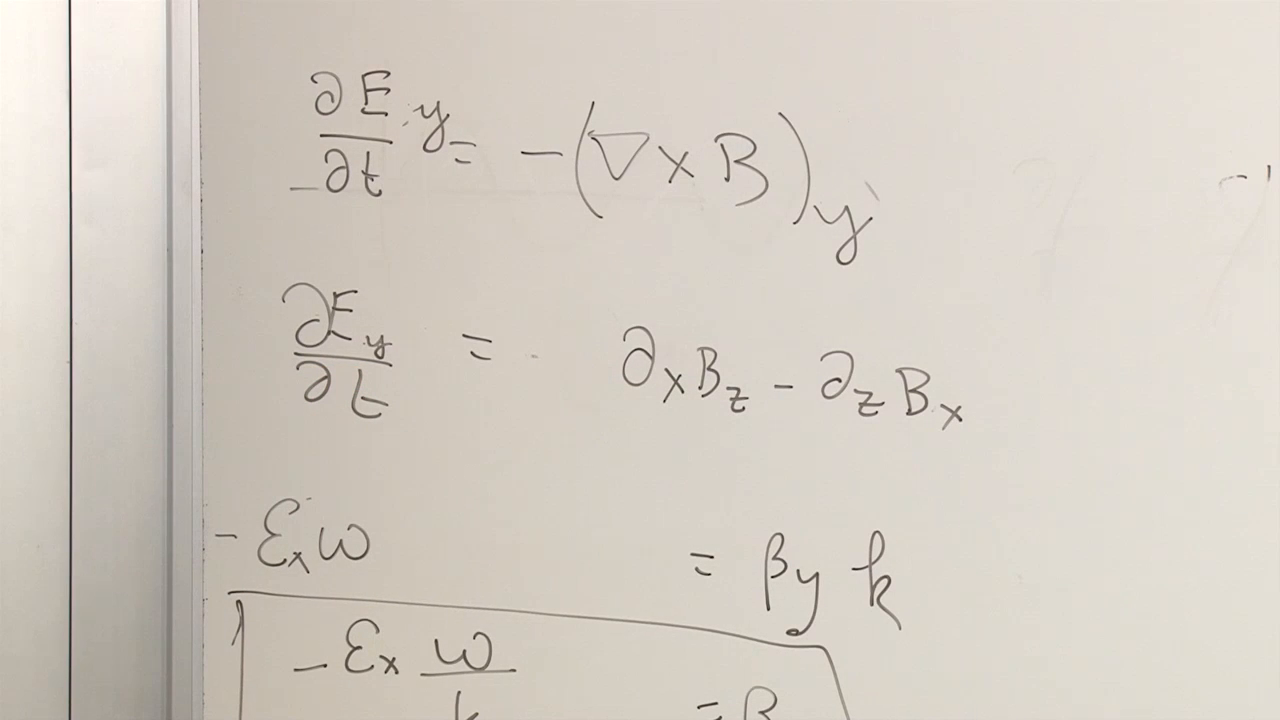
\includegraphics[width=\linewidth]{lecture_09_figure_04.png}
\caption{成分ごとの回転の計算は\(\epsilon_x\)を\(\beta_y\)と関係づけ、残っていた磁場の振幅を消去する。}
\par\smallskip
\textit{講義フレーム：00:20:15。}
\end{figure}

したがって幾何学的配置は固定される：
\begin{equation}
\mathbf E\parallel\hat{\mathbf x},
\qquad
\mathbf B\parallel\hat{\mathbf y},
\qquad
\mathbf k\parallel\hat{\mathbf z}.
\end{equation}
電場、磁場、進行方向は互いに直交する。

\begin{figure}[H]
\centering
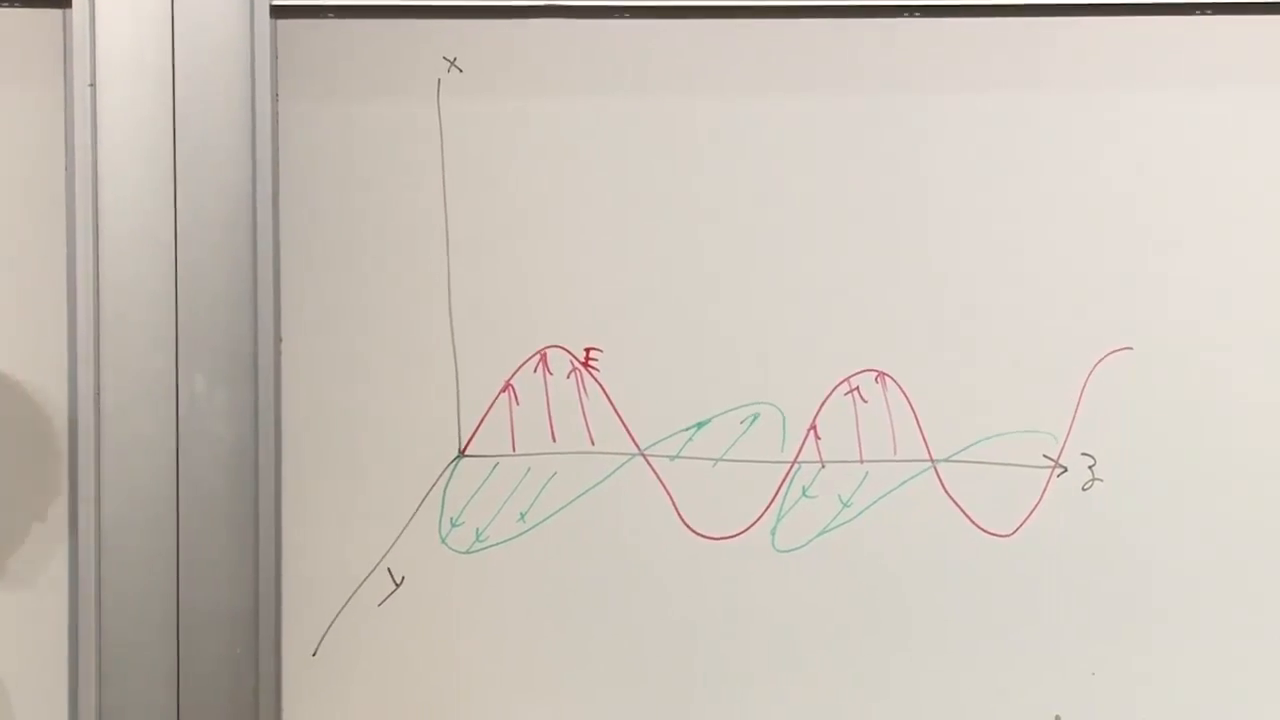
\includegraphics[width=0.94\linewidth]{lecture_09_figure_05.png}
\caption{横方向の電気振動と磁気振動が\(z\)軸に沿って進む様子を板書した図。}
\par\smallskip
\textit{講義フレーム：00:23:15。}
\end{figure}

もう一方の回転の式は独立な振幅の関係を与える。その\(y\)成分は
\begin{equation}
\dot B_y=(\nabla\times\mathbf E)_y=\partial_zE_x,
\end{equation}
であり、したがって
\begin{align}
-\omega\beta_y\cos\theta
&=
k\epsilon_x\cos\theta,
\nonumber\\
\epsilon_x
&=
-\,\beta_y\frac{\omega}{k}.
\label{eq:epsilon-beta-y}
\end{align}

\begin{figure}[H]
\centering
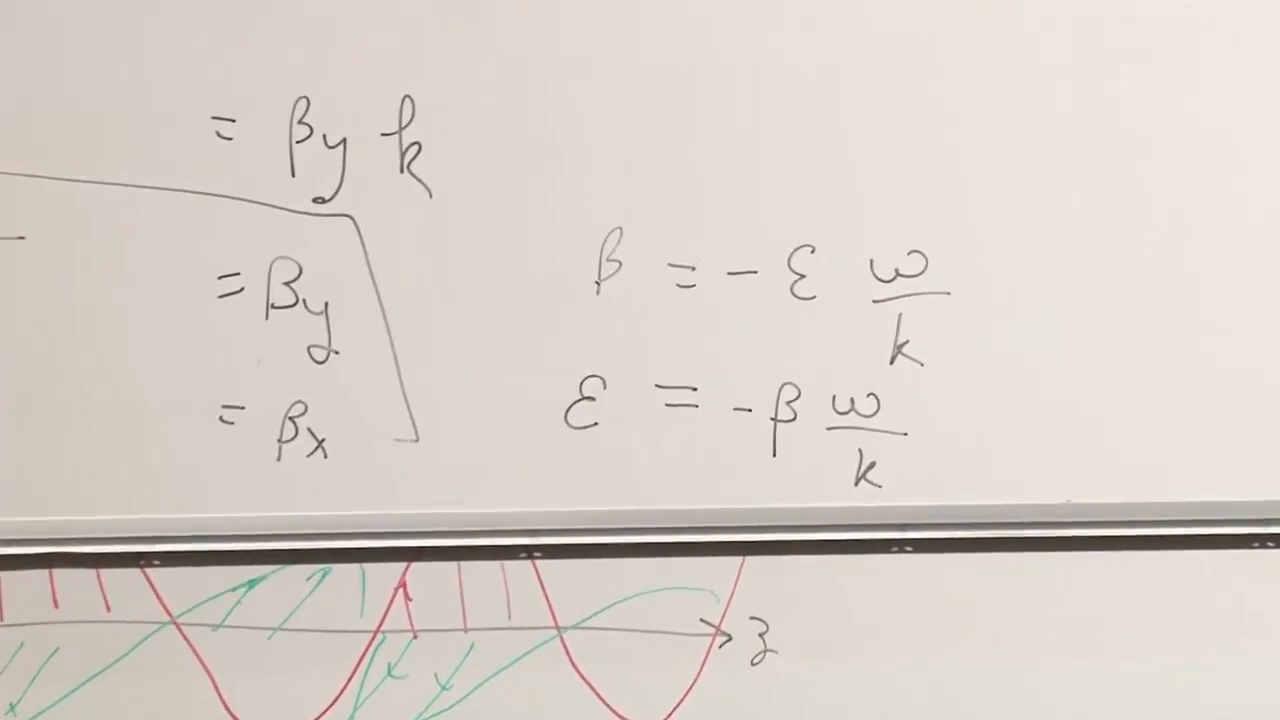
\includegraphics[width=\linewidth]{lecture_09_figure_06.png}
\caption{横波のスケッチの上に示された逆数の振幅関係。}
\par\smallskip
\textit{講義フレーム：00:25:00。}
\end{figure}

式\eqref{eq:beta-y-epsilon}と\eqref{eq:epsilon-beta-y}を組み合わせると分散関係
\begin{equation}
\left(\frac{\omega}{k}\right)^2=1.
\end{equation}
が得られる。選んだ向きに進む正振動数の波に対して
\begin{equation}
\omega=k
\qquad
(c=1).
\label{eq:omega-k}
\end{equation}
したがって共通の位相は
\begin{equation}
\theta=k(z-t).
\end{equation}
となる。通常の単位に戻すと
\begin{equation}
\omega=ck,
\qquad
\theta=k(z-ct).
\label{eq:restore-c-wave}
\end{equation}
となる。ゆえに波形は光速で剛体的に移動する。板書で用いた単位では、電場と磁場の振幅は等しい大きさをもつ。それらの相対的な負符号は向きの規約である。すなわち、選んだ\(y\)軸がどちらを向くかを述べているのであって、一方の場が他方より四分の一周期遅れているということではない。

\begin{figure}[H]
\centering
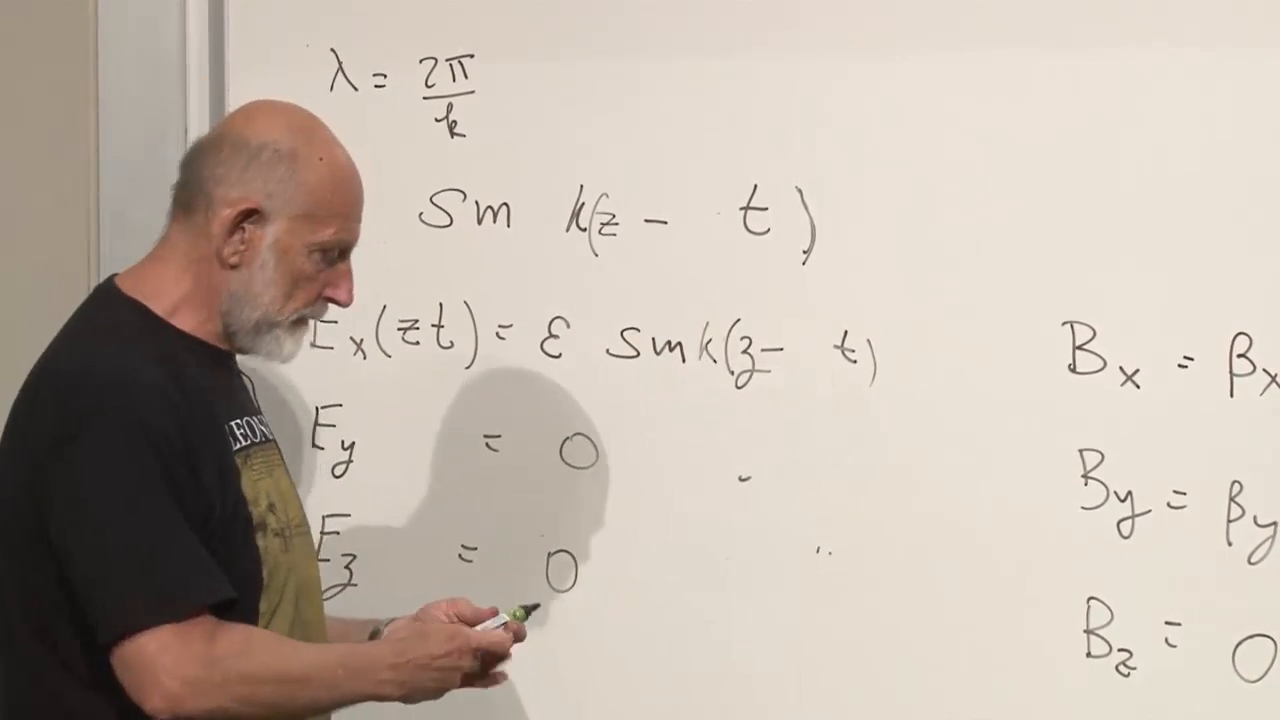
\includegraphics[width=\linewidth]{lecture_09_figure_07.png}
\caption{\(\omega=k\)を課した後の最終的な平面波の形。}
\par\smallskip
\textit{講義フレーム：00:26:45。}
\end{figure}

\begin{classroomqa}
\audiencequestion{\(\omega\)と\(k\)は異なる単位をもつのではないですか。}
\lecturerresponse{通常の単位ではそのとおりである。\(\omega\)は時間の逆数であり、\(k\)は長さの逆数である。\(c=1\)とすると、時間と長さは同じ単位をもつ。\(c\)を復元すると\(\omega=k\)は\(\omega=ck\)に変わり、これは次元解析が要求するとおりである。\lecturetimestamp{00:25:55}}
\end{classroomqa}

\begin{classroomqa}
\audiencequestion{平面波では電場と磁場は常に同位相なのですか。}
\lecturerresponse{それらは同じ位相依存性をもつ。それらの符号付き振幅は負符号だけ異なることがあり、それは\(180^\circ\)の反転と表現されることもあるが、マクスウェル方程式はこの直線偏光平面波に対して\(90^\circ\)のサイン--コサインの遅れを許さない。円偏光は横成分から組み立てられ、より注意深い言葉遣いを要するが、この成分ごとのマクスウェル関係を変えるものではない。\lecturetimestamp{00:27:31}}
\end{classroomqa}

\begin{classroomqa}
\audiencequestion{両方の場が同時にゼロを通過するなら、エネルギーは依然として保存されるのですか。}
\lecturerresponse{はい。一つの固定点におけるエネルギー密度は波が通過するにつれて振動するが、エネルギーは消えたのではなく移動したのである。ある時刻に一つの領域を占めていたものは、少し後の時刻には隣接する領域を占める。ポインティング流束によってより完全に表される局所的なエネルギー輸送が、変化する密度と保存を両立させる。\lecturetimestamp{00:28:15}}
\end{classroomqa}

マクスウェル方程式は線形である。振幅\(\epsilon_x\)は大きくても小さくてもよく、\(\beta_y\)はそれから従い、解の任意の和や差もまた解である。したがって異なる向きに進む波を重ね合わせることができる。この短い計算は行う価値がある。電磁気学の説明が電磁波を未説明の引用として残すべきではないからである。

\begin{classroomqa}
\audiencequestion{この導出では、最初から\(\mathbf E\)と\(\mathbf B\)が同じ位相をもつと仮定していたのですか。}
\lecturerresponse{共通の位相はアンザッツとして書かれたが、それは独立な物理的仮定ではない。回転の式の各辺が場を微分するため、方程式は自明でない相対位相を消去する。その後、共通の位相のずれは原点の平行移動によって取り除くことができる。\lecturetimestamp{00:29:56}}
\end{classroomqa}

\begin{classroomqa}
\audiencequestion{第二の関係\(\epsilon_x=-\beta_y\omega/k\)はどこから来たのですか。}
\lecturerresponse{第一の関係は\(\dot{\mathbf E}=-\nabla\times\mathbf B\)から来た。第二の関係は、同じ成分計算で\(\mathbf E\)と\(\mathbf B\)を入れ替えた相方の式\(\dot{\mathbf B}=\nabla\times\mathbf E\)から来る。\(\omega^2=k^2\)を得るには両方が必要である。\lecturetimestamp{00:30:25}}
\end{classroomqa}

\section{なぜ微分方程式だけでは十分でないか}

ここで、特定の解から理論の構造へと目を向ける。最小作用の原理こそが、エネルギー保存、運動量保存、およびそれらと時空対称性との関係を組織するものである。保存に値するエネルギーも有用な対称性原理ももたない微分方程式を考案することはできる。しかしマクスウェル方程式はむしろラグランジアンから生じるべきである。

動的な族のみを生成する必要がある：
\begin{equation}
\partial_\mu F^{\mu\nu}=J^\nu.
\label{eq:target-sourced-maxwell}
\end{equation}
Bianchi 族はすでに \(F_{\mu\nu}\) の定義から従う。
三ベクトル言語では、我々の規約により
\begin{align}
\nabla\cdot\mathbf E&=\rho,
\label{eq:gauss-source}
\\
\dot{\mathbf E}+\nabla\times\mathbf B&=-\,\mathbf J.
\label{eq:ampere-course-sign}
\end{align}
\eqref{eq:ampere-course-sign} のマイナス符号は重要である。これは \eqref{eq:course-f-convention} の下での \eqref{eq:target-sourced-maxwell} の成分形であり、終盤のライブ符号チェックで再発見されるであろう。

\begin{figure}[H]
\centering
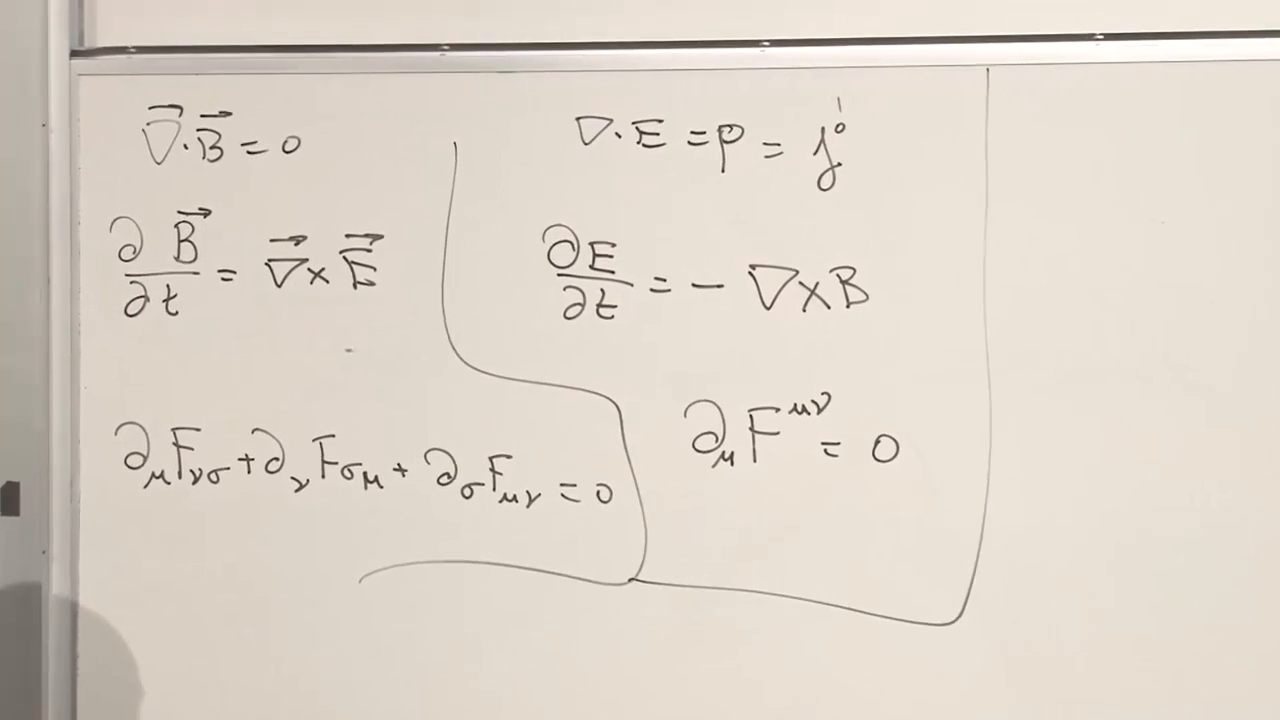
\includegraphics[width=\linewidth]{lecture_09_figure_08.png}
\caption{波動解から作用原理への移行における完全な Maxwell 板。}
\par\smallskip
\textit{講義フレーム：00:32:45。}
\end{figure}

\section{局所相対論的場の理論}

第一の原理は局所性である。作用とは、同一時空点における場とその一階導関数から構成される密度の時空にわたる積分である：
\begin{equation}
S=\int d^4x\,\mathcal L(\phi,\phi_{,\mu}),
\qquad
\phi_{,\mu}\equiv\partial_\mu\phi.
\label{eq:local-action}
\end{equation}
コンマは簡潔な導関数記法である。第二の原理は Lorentz 不変性である：\(\mathcal L\) はスカラーでなければならない。

\subsection{スカラー場による予行演習}

四元ベクトルを変分する前に、一つのスカラー場でこの方法を予行演習しよう。局所 Lorentz スカラーはポテンシャル \(U(\phi)\) および二つの導関数の縮約に依存しうる：
\begin{equation}
\mathcal L_\phi
=
-\frac12\,\partial_\mu\phi\,\partial^\mu\phi-U(\phi).
\label{eq:scalar-lagrangian}
\end{equation}
mostly-plus 計量では、
\begin{equation}
\partial_\mu\phi\,\partial^\mu\phi
=
-\dot\phi^{\,2}+|\nabla\phi|^2,
\end{equation}
したがって
\begin{equation}
\mathcal L_\phi
=
\frac12\dot\phi^{\,2}
-\frac12|\nabla\phi|^2
-U(\phi).
\end{equation}
上げた時間導関数は下げたものと符号が異なる；上げた空間導関数と下げた空間導関数は異ならない。

\begin{classroomqa}
\audiencequestion{導関数の添字を下ではなく上に置くことに意味はあるのか？}
\lecturerresponse{はい。添字を上げることは逆計量との縮約である。符号 \((-+++)\) では、
\(\partial^0=-\partial_0\) である一方、
\(\partial^i=\partial_i\) である。だから時間導関数の項が三つの空間項と反対の符号を帯びるのである。
\lecturetimestamp{00:38:02}}
\end{classroomqa}

場の Euler--Lagrange 方程式は
\begin{equation}
\partial_\mu\left(
\frac{\partial\mathcal L}{\partial\phi_{,\mu}}
\right)
=
\frac{\partial\mathcal L}{\partial\phi}.
\label{eq:field-el}
\end{equation}
\eqref{eq:scalar-lagrangian} に対して、
\begin{equation}
\frac{\partial\mathcal L_\phi}{\partial\phi_{,\mu}}
=
-\partial^\mu\phi,
\qquad
\frac{\partial\mathcal L_\phi}{\partial\phi}
=
-U'(\phi),
\end{equation}
したがって
\begin{equation}
\Box\phi=U'(\phi),
\qquad
\Box\equiv\partial_\mu\partial^\mu.
\end{equation}
等価的に、
\begin{equation}
\ddot\phi-\nabla^2\phi=-U'(\phi).
\label{eq:scalar-wave}
\end{equation}
板書では \(x\) 導関数のみが \(y\) および \(z\) 項の前に書かれ、それらは暗黙に残される。結果はポテンシャルからの力を持つおなじみの波動方程式である。

\begin{figure}[H]
\centering
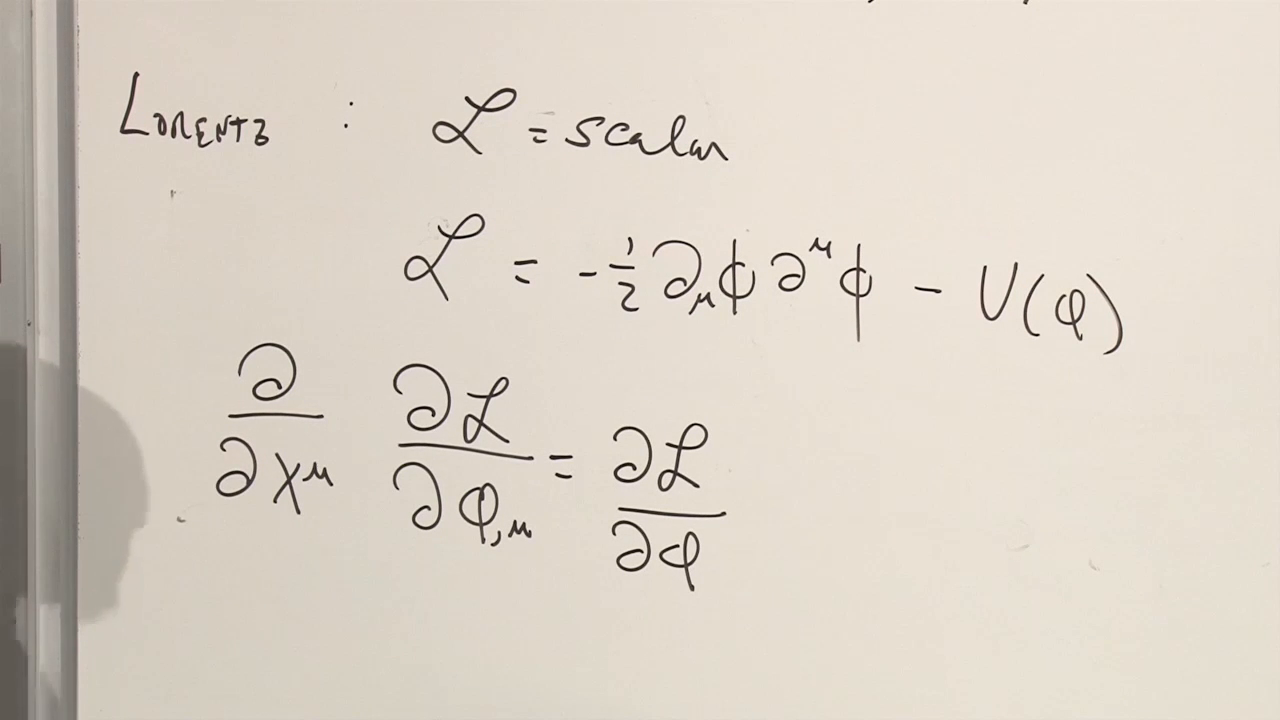
\includegraphics[width=\linewidth]{lecture_09_figure_09.png}
\caption{局所性、スカラー Lorentz 不変 Lagrange 関数、および場の理論の Euler--Lagrange 方程式。}
\par\smallskip
\textit{講義フレーム：00:41:00。}
\end{figure}

電磁気学の計算は、四つの場とより多くの添字を伴う同じ変分過程である。

\section{ゲージ不変性が Maxwell スカラーを選び出す}

第三の原理を加える：ゲージ不変性。当面 \(J^\mu=0\) とし、自由場を考える。ゲージ変換は
\begin{equation}
A_\mu\longrightarrow A_\mu+\partial_\mu\chi.
\label{eq:gauge-transform}
\end{equation}
混合二階導関数が可換であるため、場のテンソルは変化しない：
\begin{align}
F_{\mu\nu}
&\longrightarrow
F_{\mu\nu}
+\partial_\mu\partial_\nu\chi
-\partial_\nu\partial_\mu\chi
\nonumber\\
&=F_{\mu\nu}.
\end{align}

Lorentz 不変性のみではスカラー
\begin{equation}
A_\mu A^\mu.
\end{equation}
が許されるであろう。それにもかかわらず、これは \eqref{eq:gauge-transform} の下で変化するため Maxwell 理論では禁じられる。この式の添字は場の成分をラベルするものであり、導関数ではない。導関数は \(A_{\nu,\mu}=\partial_\mu A_\nu\) のようにコンマで示される。

\begin{figure}[H]
\centering
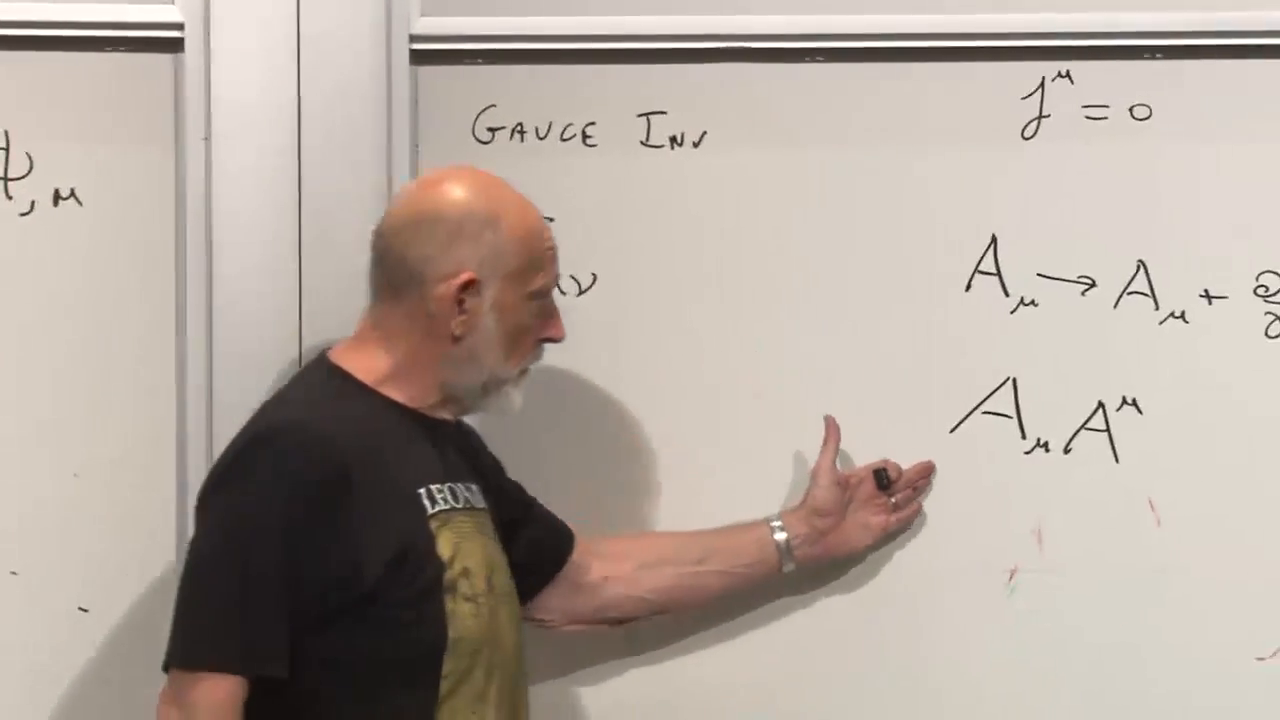
\includegraphics[width=\linewidth]{lecture_09_figure_10.png}
\caption{ゲージ変換と Lorentz スカラー
\(A_\mu A^\mu\)。これはゲージ不変でないため棄却される。}
\par\smallskip
\textit{講義フレーム：00:43:40。}
\end{figure}

したがって我々は \(F_{\mu\nu}\) から自由 Lagrange 関数を構成すべきである。線形トレースは失敗する：
\begin{equation}
F^\mu{}_\mu=0.
\end{equation}
反対称性によりすべての対角成分が消える：
\begin{equation}
F_{00}=F_{11}=F_{22}=F_{33}=0.
\end{equation}
添字を上げることは符号を変えうるが、ゼロを何か他のものに変えることはできない。

\begin{figure}[H]
\centering
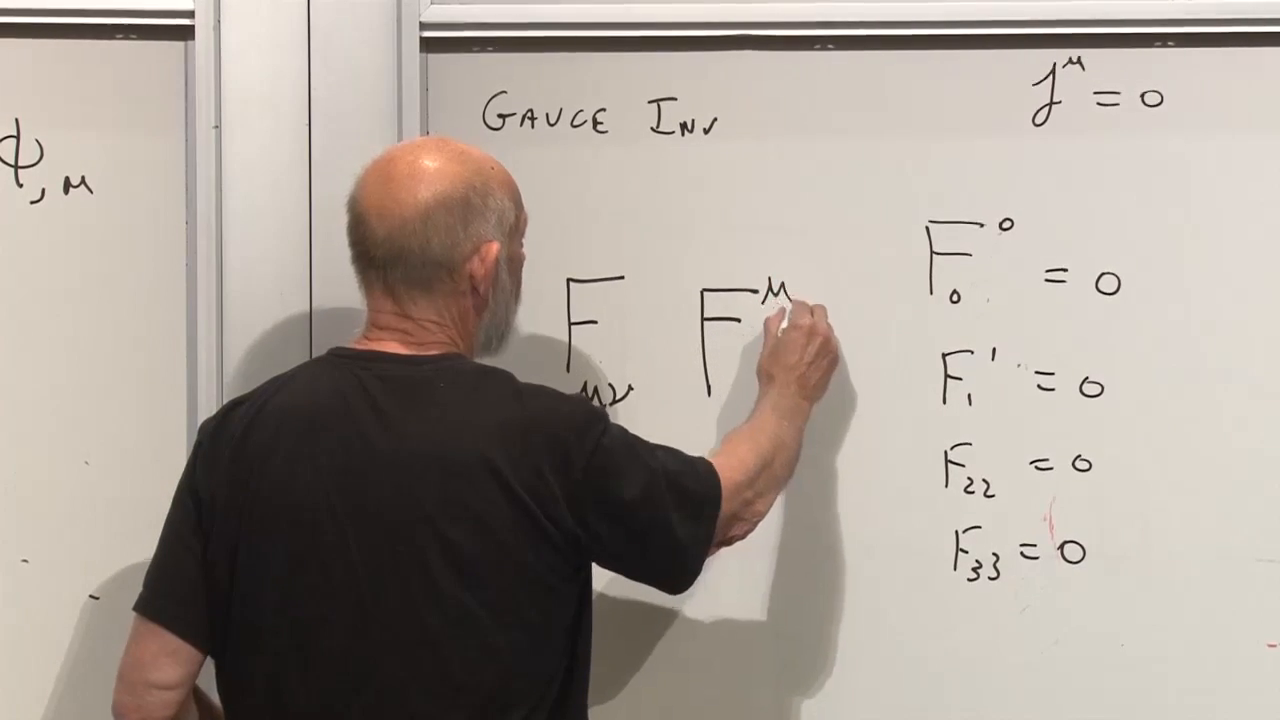
\includegraphics[width=\linewidth]{lecture_09_figure_11.png}
\caption{試みられた線形トレースと、反対称場のテンソルの消える対角成分。}
\par\smallskip
\textit{講義フレーム：00:47:00。}
\end{figure}

最初の非零 Lorentz スカラーは二次である：
\begin{equation}
F_{\mu\nu}F^{\mu\nu}.
\label{eq:f2-scalar}
\end{equation}
これを引用するのではなく縮約を解き明かそう。混合成分は電場を含む。その時間添字を上げるとマイナス符号が寄与し、両方の順序 \(0i\) と \(i0\) が現れる：
\begin{equation}
\sum_i\left(F_{0i}F^{0i}+F_{i0}F^{i0}\right)
=-2E^2.
\end{equation}
純粋に空間的な成分は磁場を含む。空間添字を上げても符号は変化せず、再び両方の順序が現れる：
\begin{equation}
\sum_{i<j}\left(F_{ij}F^{ij}+F_{ji}F^{ji}\right)
=2B^2.
\end{equation}
したがって
\begin{equation}
F_{\mu\nu}F^{\mu\nu}=2(B^2-E^2),
\qquad
-F_{\mu\nu}F^{\mu\nu}=2(E^2-B^2).
\label{eq:f2-eb}
\end{equation}

\begin{figure}[H]
\centering
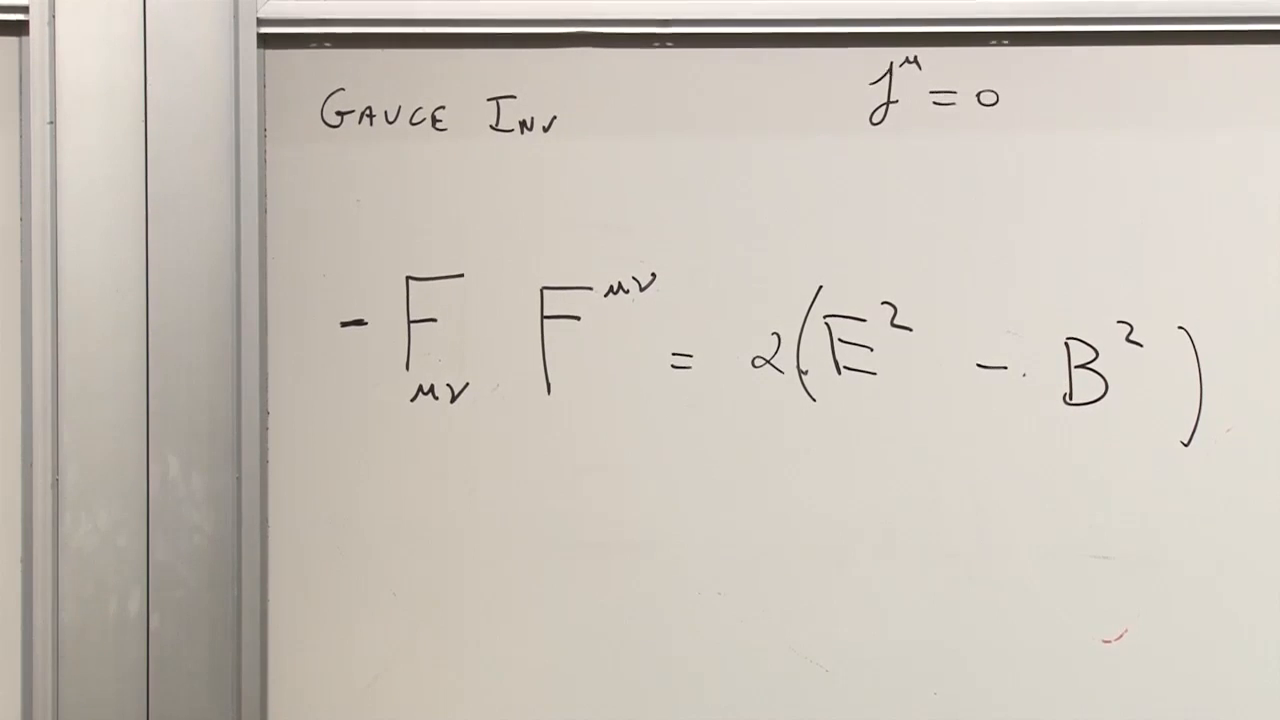
\includegraphics[width=\linewidth]{lecture_09_figure_12.png}
\caption{電場と磁場の大きさで表した完成した縮約。}
\par\smallskip
\textit{講義フレーム：00:51:00。}
\end{figure}

\begin{classroomqa}
\audiencequestion{\(F_{00}\) もまたゼロか？}
\lecturerresponse{はい。反対称テンソルのすべての対角成分は消え、\(F_{00}\) も含まれる。\(\mathbf E\) を符号化する非対角混合成分と、\(\mathbf B\) を符号化する非対角空間成分のみが寄与する。
\lecturetimestamp{00:51:36}}
\end{classroomqa}

従来の規格化は
\begin{equation}
\boxed{
\mathcal L_{\mathrm{EM}}
=
-\frac14F_{\mu\nu}F^{\mu\nu}
}
\label{eq:maxwell-lagrangian}
\end{equation}
または
\begin{equation}
\mathcal L_{\mathrm{EM}}
=
\frac12(E^2-B^2).
\label{eq:maxwell-lagrangian-eb}
\end{equation}
である。マイナス符号により電気項がおなじみの正符号をとる。因子\(1/4\)は、各反対称対が二度現れることを補償し、従来の因子\(1/2\)を残す。自由作用全体に非零定数を掛けても源のない方程式は変わらないが、この規格化が標準的な源結合に適合するものである。

\section{自由電磁場の変分}

独立な場は
\begin{equation}
A_0,\qquad A_x,\qquad A_y,\qquad A_z.
\end{equation}
である。各成分\(A_\nu\)に対し、オイラー--ラグランジュ方程式は
\begin{equation}
\partial_\mu\left(
\frac{\partial\mathcal L}{\partial A_{\nu,\mu}}
\right)
=
\frac{\partial\mathcal L}{\partial A_\nu},
\qquad
A_{\nu,\mu}\equiv\partial_\mu A_\nu.
\label{eq:vector-el-comma}
\end{equation}
である。コンマ記法における配置はゆっくり読む価値がある。第一の添字は\(A\)のどの成分が場であるかを示し、第二の添字は微分する座標を示す。

この記法では、
\begin{equation}
F_{\mu\nu}
=
A_{\nu,\mu}-A_{\mu,\nu}.
\label{eq:f-comma-consistent}
\end{equation}
である。これはまさに\eqref{eq:course-f-convention}である。コンマ添字を逆の語順で書くと中間のマイナス符号が変わる。それゆえ成分計算が有用なのである。

\begin{figure}[H]
\centering
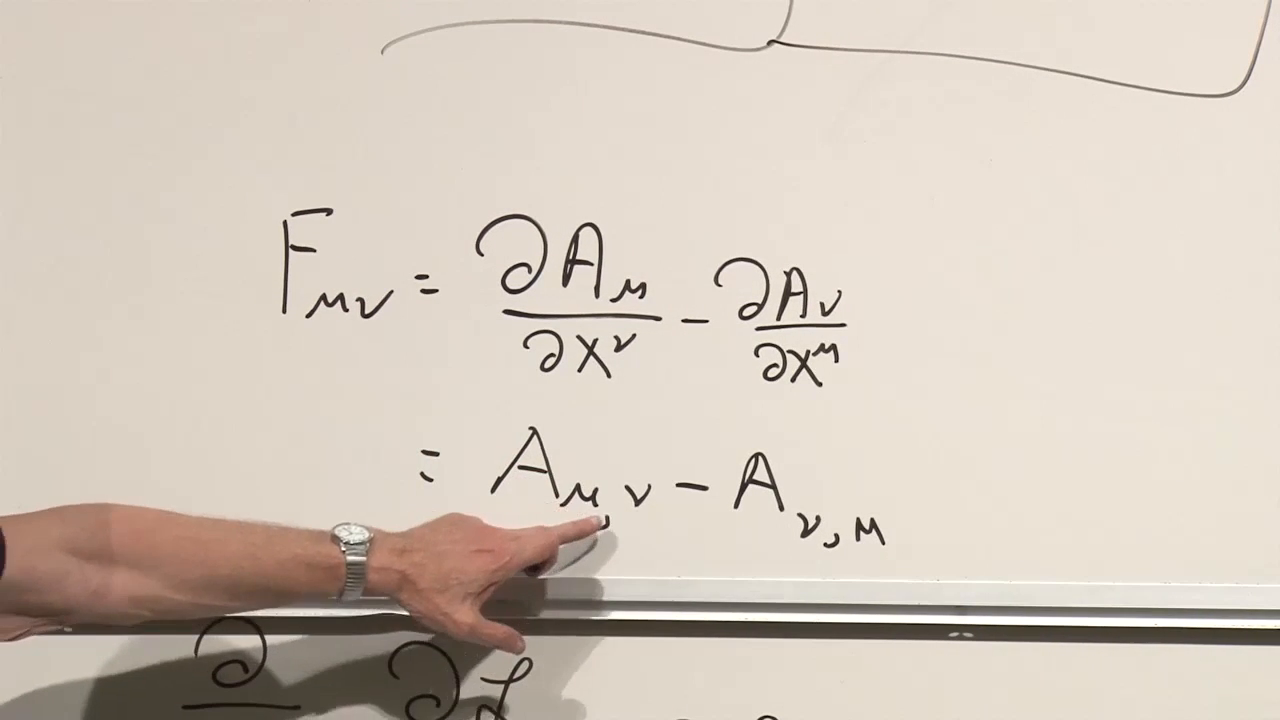
\includegraphics[width=\linewidth]{lecture_09_figure_13.png}
\caption{四つのポテンシャル成分を独立な場として同定した後、コンマ記法で表した場のテンソル。}
\par\smallskip
\textit{講義フレーム：00：55：30。}
\end{figure}

\begin{figure}[H]
\centering
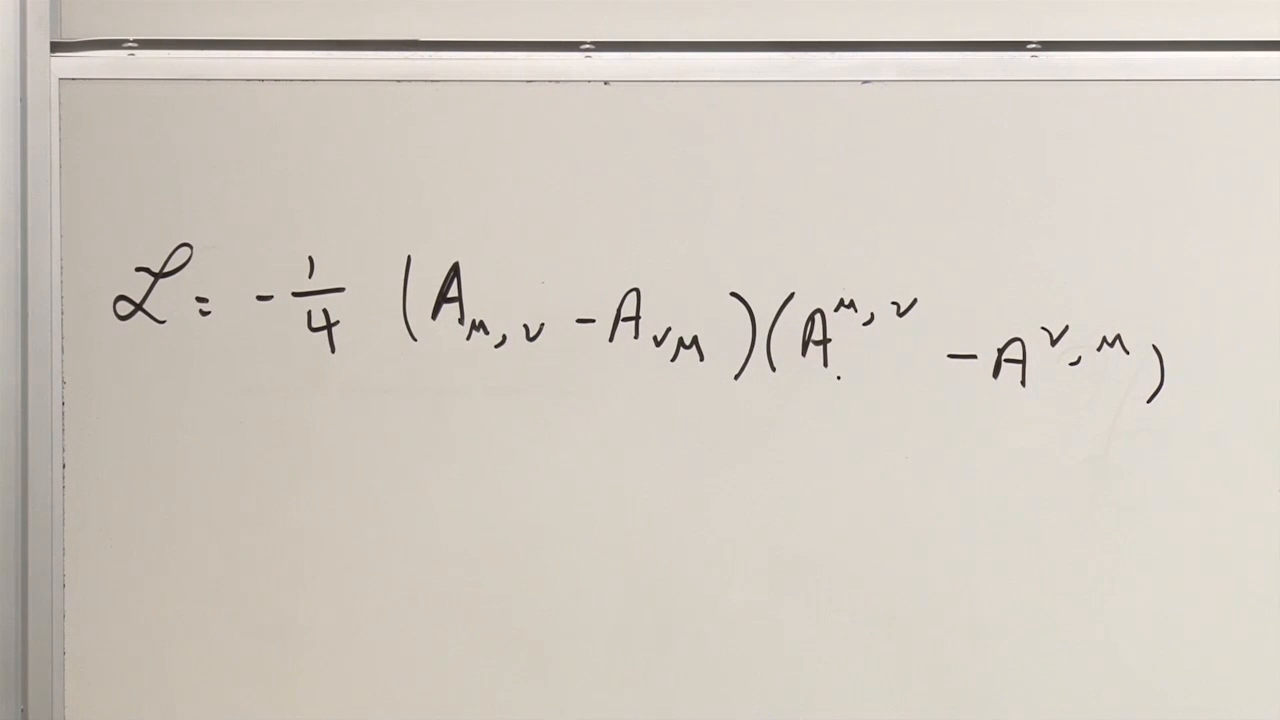
\includegraphics[width=\linewidth]{lecture_09_figure_14.png}
\caption{ベクトルポテンシャルの微分で陽に表したマクスウェルラグランジアン。}
\par\smallskip
\textit{講義フレーム：00：56：45。}
\end{figure}

\subsection{一つの代表的な微分}

微分\(A_{x,y}=\partial_yA_x\)を選ぶ。完全な和における\(xy\)項と\(yx\)項は
\begin{align}
\mathcal L_{\mathrm{EM}}
&\supset
-\frac14\left(F_{xy}F^{xy}+F_{yx}F^{yx}\right)
\nonumber\\
&=
-\frac12F_{xy}^2
\nonumber\\
&=
-\frac12\left(A_{x,y}-A_{y,x}\right)^2.
\label{eq:isolated-xy-piece}
\end{align}
に寄与する。最後の等号は、二乗すると符号が消えるため安全である：
\(A_{x,y}-A_{y,x}=F_{yx}=-F_{xy}\)。

\begin{figure}[H]
\centering
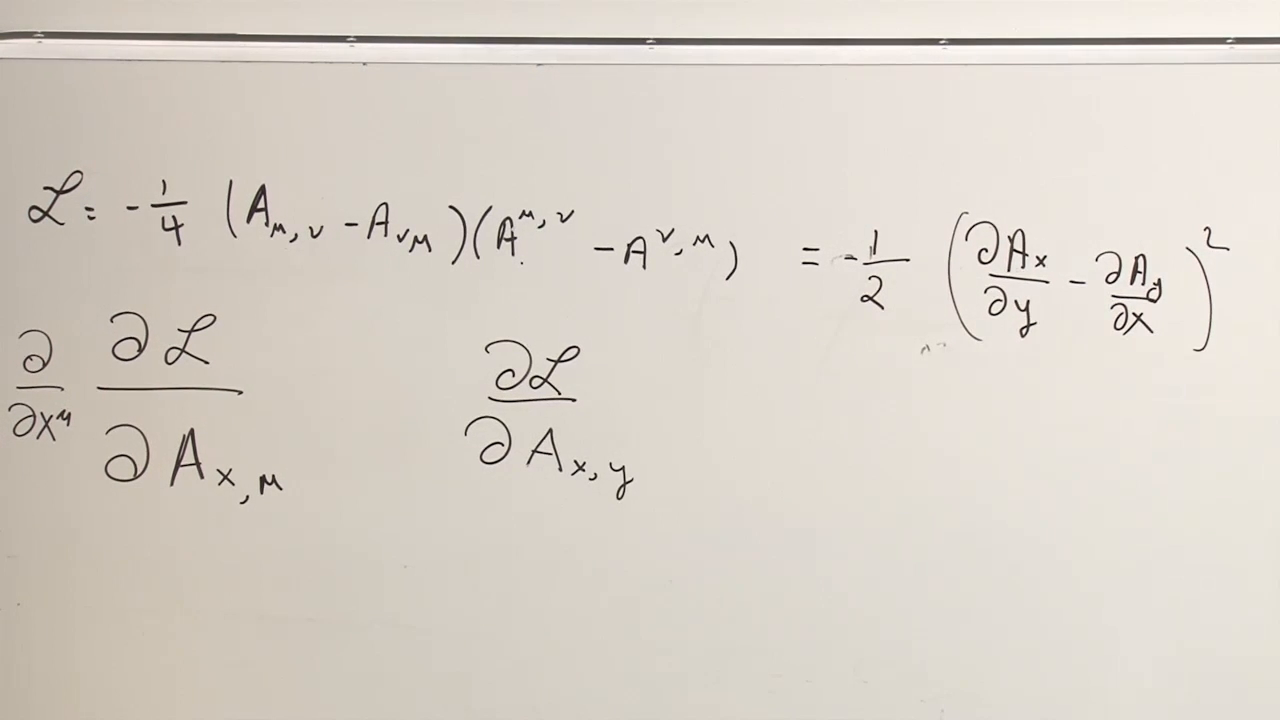
\includegraphics[width=\linewidth]{lecture_09_figure_15.png}
\caption{代表的な\(A_{x,y}\)微分と、分離された反対称二乗。}
\par\smallskip
\textit{講義フレーム：01：00：45。}
\end{figure}

微分する：
\begin{align}
\frac{\partial\mathcal L_{\mathrm{EM}}}
{\partial A_{x,y}}
&=
-\left(A_{x,y}-A_{y,x}\right)
\nonumber\\
&=
F_{xy}.
\label{eq:component-variation}
\end{align}
黒板では、添字が黒板の微分順序に従うテンソルにマイナス符号を付けてこれを要約している。コース全体の定義\eqref{eq:course-f-convention}を用いると、不変な形の主張は
\begin{equation}
\frac{\partial\mathcal L_{\mathrm{EM}}}
{\partial(\partial_\mu A_\nu)}
=
-F^{\mu\nu}.
\label{eq:maxwell-canonical-derivative}
\end{equation}
である。例\(\partial_yA_x\)に対しては、これは
\(-F^{yx}=F^{xy}\)を与え、まさに
\eqref{eq:component-variation}である。したがって、見かけの符号の違いは添字順序の記帳上の問題にすぎない。

\begin{figure}[H]
\centering
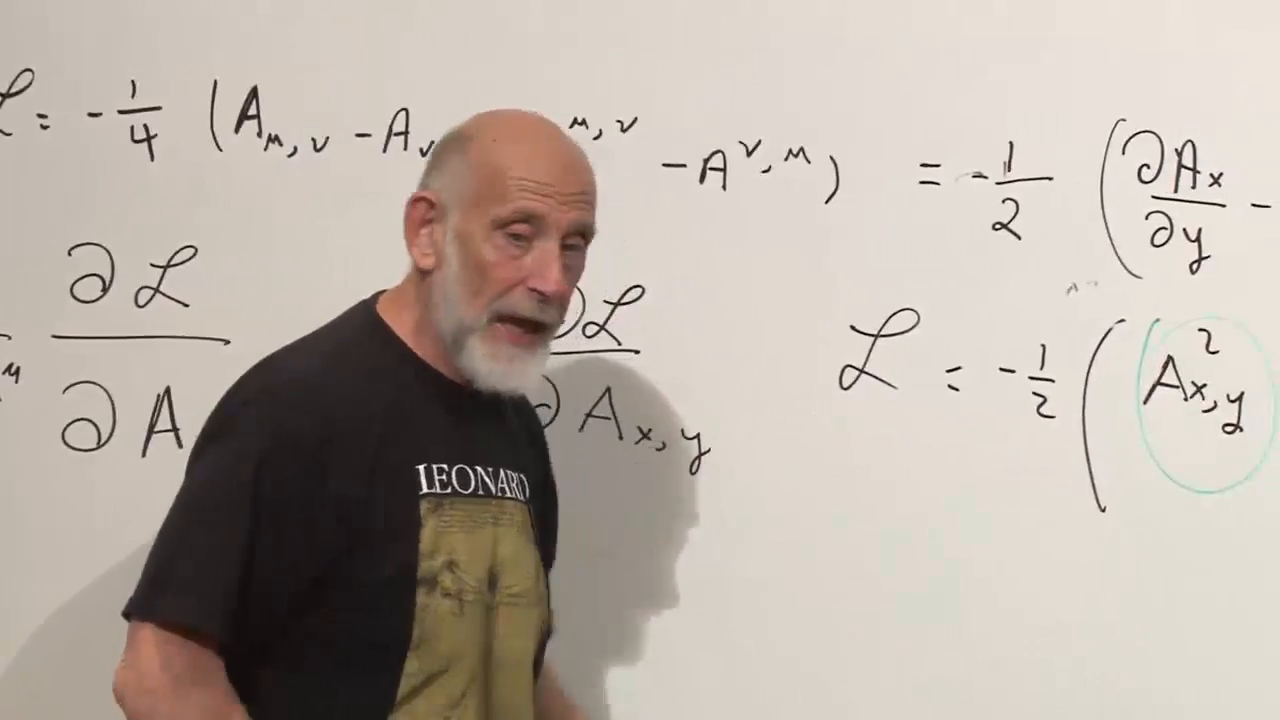
\includegraphics[width=\linewidth]{lecture_09_figure_16.png}
\caption{ポテンシャルの一つの微分に関して微分する前の、選ばれた二乗の展開。}
\par\smallskip
\textit{講義フレーム：01：03：00。}
\end{figure}

\begin{classroomqa}
\audiencequestion{成分微分における因子\(1/2\)はどうなったのか。}
\lecturerresponse{二乗を微分すると因子2が生じ、それが\(1/2\)を打ち消す：
\[
\frac{d}{dx}\left[-\frac12x^2\right]=-x.
\]
先の\(1/4\)から\(1/2\)への変化は、二つの順序付けられたテンソル成分\(xy\)と\(yx\)から来た。\lecturetimestamp{01:03:29}}
\end{classroomqa}

真空ラグランジアンには微分されないポテンシャルは存在しない：
\begin{equation}
\frac{\partial\mathcal L_{\mathrm{EM}}}{\partial A_\nu}=0.
\end{equation}
\eqref{eq:vector-el-comma}に代入すると
\begin{equation}
-\partial_\mu F^{\mu\nu}=0,
\end{equation}
または等価に
\begin{equation}
\boxed{\partial_\mu F^{\mu\nu}=0.}
\label{eq:free-maxwell-from-action}
\end{equation}
が得られる。

\begin{figure}[H]
\centering
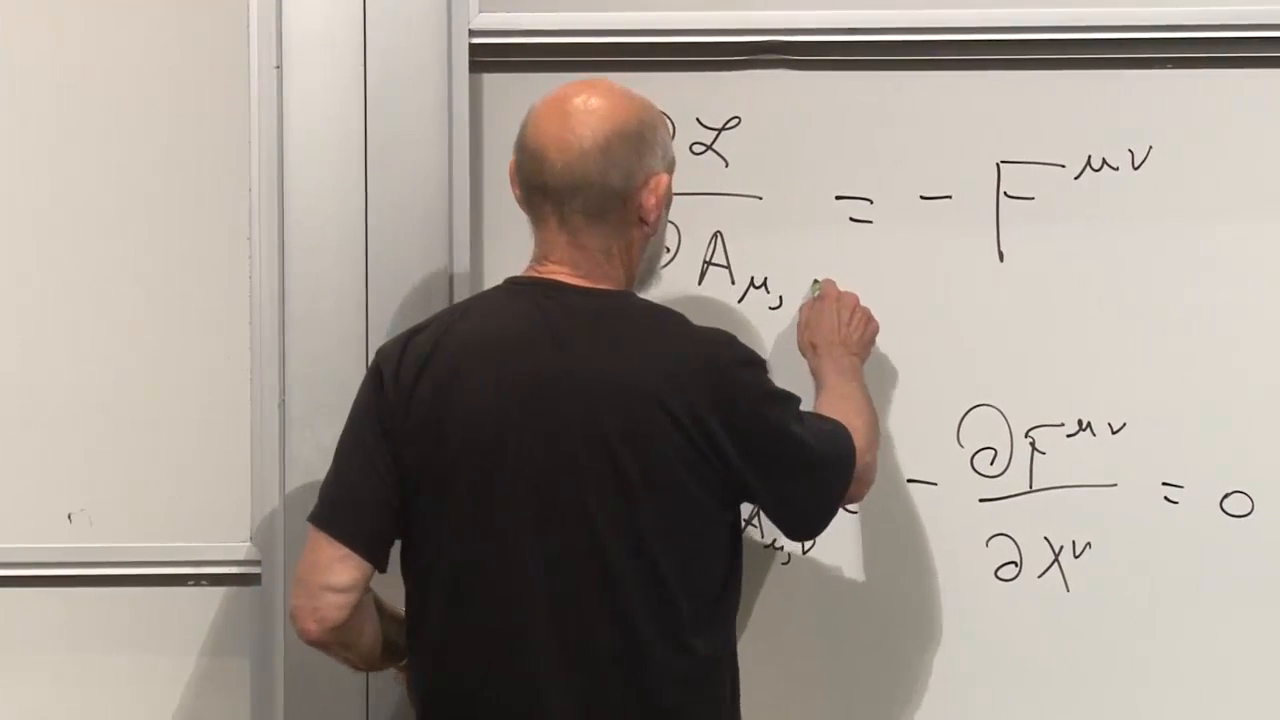
\includegraphics[width=\linewidth]{lecture_09_figure_17.png}
\caption{成分の結果を一般化し、オイラー--ラグランジュ方程式に代入したもの。}
\par\smallskip
\textit{講義フレーム：01：09：00。}
\end{figure}

同じ結論は作用全体を変分する方がより簡潔に導かれる：
\begin{align}
\delta S_{\mathrm{EM}}
&=
-\frac12\int d^4x\,
F^{\mu\nu}
\left(\partial_\mu\delta A_\nu
-\partial_\nu\delta A_\mu\right)
\nonumber\\
&=
-\int d^4x\,F^{\mu\nu}\partial_\mu\delta A_\nu
\nonumber\\
&=
\int d^4x\,
\left(\partial_\mu F^{\mu\nu}\right)\delta A_\nu,
\label{eq:global-maxwell-variation}
\end{align}
ここで境界項は捨てられる。反対称性が第一行の二つの項をまとめる。\(\delta A_\nu\)は任意であるから、
\eqref{eq:free-maxwell-from-action}
が従う。

\begin{classroomqa}
\audiencequestion{分離された二乗は、磁場が\(z\)方向のみを向くと仮定していたのか。}
\lecturerresponse{いいえ。それは検討のために完全な和から取り出した一つの項にすぎず、その後に省略記号が続くべきである。残りの空間的対は他の磁場成分を与え、時間--空間の対は電場成分を与える。\lecturetimestamp{01:08:05}}
\end{classroomqa}

\begin{classroomqa}
\audiencequestion{二つの空間添字の代わりに一つの時間添字を選ぶと結果は変わるのか。}
\lecturerresponse{同じ一般微分を与え、計量の符号は添字の上げ下げで処理される。二つの空間添字は磁場成分を選び、一つの時間添字と一つの空間添字は電場成分を選ぶ。反対称公式
\eqref{eq:maxwell-canonical-derivative}
は両方をカバーする。
\lecturetimestamp{01:08:46}}
\end{classroomqa}

\begin{classroomqa}
\audiencequestion{我々はまだ\(J^\mu=0\)を仮定しているのか。}
\lecturerresponse{この自由場の導出に限ってである。ゲージ不変な運動項を同定できるように、電流を一時的にゼロに置いた。ここでそれを復元し、どの余分な項がマクスウェル方程式の右辺を生むかを問う。\lecturetimestamp{01:09:41}}
\end{classroomqa}

代数は難しくないが、ただ眺めるのではなく、実際に手を動かして計算しなければならない。添字の連鎖を一度たどっただけでは身につかない。自分の手でその連鎖を再現してこそ定着する。

\section{保存された四元電流}

源は四元電流
\begin{equation}
J^\mu=(\rho,\mathbf J).
\end{equation}
である。その時間成分は電荷密度であり、空間成分は互いに直交する三つの窓を通る電荷の流束である。等価な言い方をすれば、小さな固定された箱について
\begin{equation}
\frac{\partial\rho}{\partial t}
+\nabla\cdot\mathbf J=0.
\label{eq:continuity-vector-l9}
\end{equation}
箱の内部の電荷は、その境界を通って流れ出ることによってのみ減少しうる。共変記法では
\begin{equation}
\boxed{\partial_\mu J^\mu=0.}
\label{eq:continuity-covariant-l9}
\end{equation}

\begin{figure}[H]
\centering
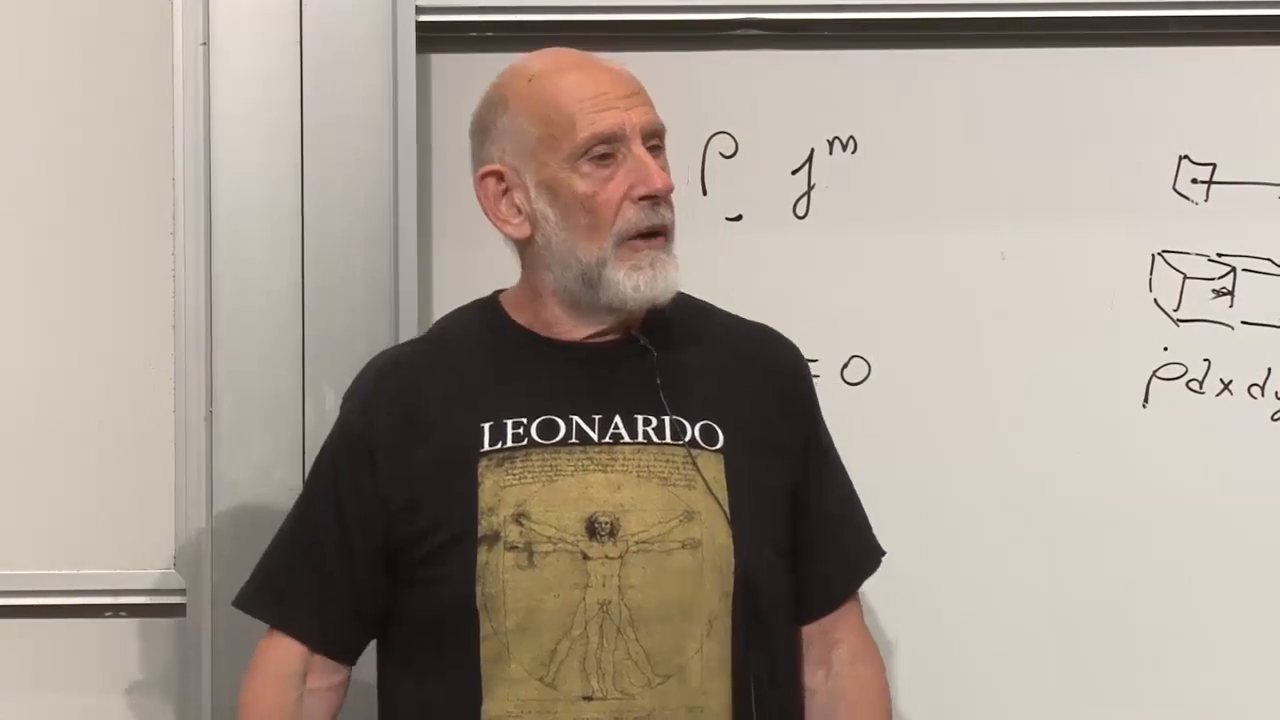
\includegraphics[width=\linewidth]{lecture_09_figure_18.png}
\caption{電荷密度、空間電流、そして源の結合を導入する前に思い出した小さな箱による解釈。}
\par\smallskip
\textit{講義フレーム: 01:14:45。}
\end{figure}

\section{源の結合とゲージ不変性}

電流とポテンシャルの両方について線形な最も単純な局所ローレンツスカラーは
\begin{equation}
S_{\mathrm{int}}
=
-\int d^4x\,J^\mu A_\mu.
\label{eq:interaction-action}
\end{equation}
である。全体の符号は慣習による。講義では、電荷の符号に関する歴史的な選択は結局ベンジャミン・フランクリンに責任があると冗談めかして言われるが、本当の要点は、一貫した符号の慣習をどこでも用いなければならないということである。

一見すると \eqref{eq:interaction-action} はゲージ不変には見えない。\eqref{eq:gauge-transform} の下で
\begin{equation}
\delta_\chi S_{\mathrm{int}}
=
-\int d^4x\,J^\mu\partial_\mu\chi.
\label{eq:gauge-variation-interaction}
\end{equation}

\begin{figure}[H]
\centering
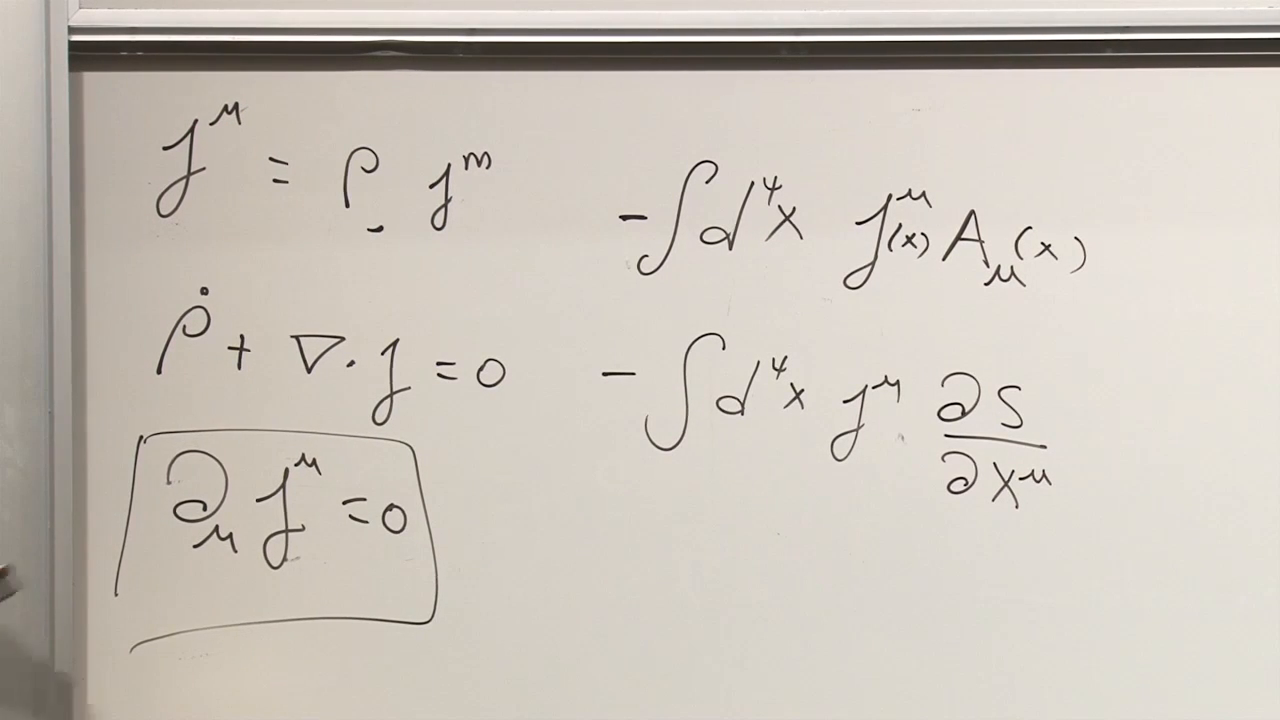
\includegraphics[width=\linewidth]{lecture_09_figure_19.png}
\caption{相互作用作用と、\(A_\mu\mapsto A_\mu+\partial_\mu\chi\) の下でのその変分。}
\par\smallskip
\textit{講義フレーム: 01:16:45。}
\end{figure}

この仕組みを初等的な言葉で見るために、縮約を展開しよう:
\begin{equation}
J^\mu\partial_\mu\chi
=
J^0\partial_0\chi
+J^1\partial_1\chi
+J^2\partial_2\chi
+J^3\partial_3\chi.
\end{equation}
電流が大きな実験室に閉じ込められているか、境界で消えるほど十分速く減衰すると仮定する。各項を部分積分する。例えば第一の空間座標については
\begin{align}
-\int d^4x\,J^1\partial_1\chi
&=
-\int dt\,dx^2\,dx^3
\left[J^1\chi\right]_{x^1=-\infty}^{x^1=+\infty}
\nonumber\\
&\quad
+\int d^4x\,\chi\,\partial_1J^1
\nonumber\\
&=
\int d^4x\,\chi\,\partial_1J^1.
\end{align}
同じ操作が時間項および残りの二つの空間項にも当てはまる。

\begin{figure}[H]
\centering
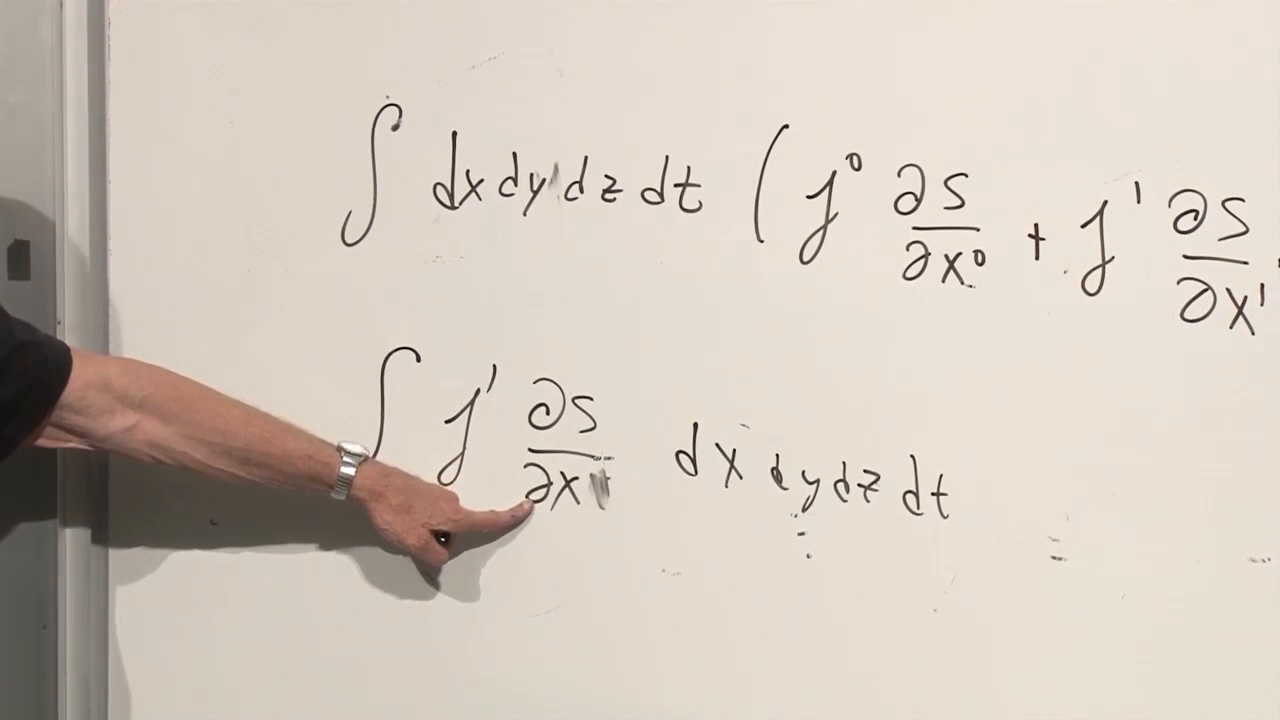
\includegraphics[width=\linewidth]{lecture_09_figure_20.png}
\caption{部分積分の前に展開された四つのゲージ変分項。}
\par\smallskip
\textit{講義フレーム: 01:19:15。}
\end{figure}

\begin{figure}[H]
\centering
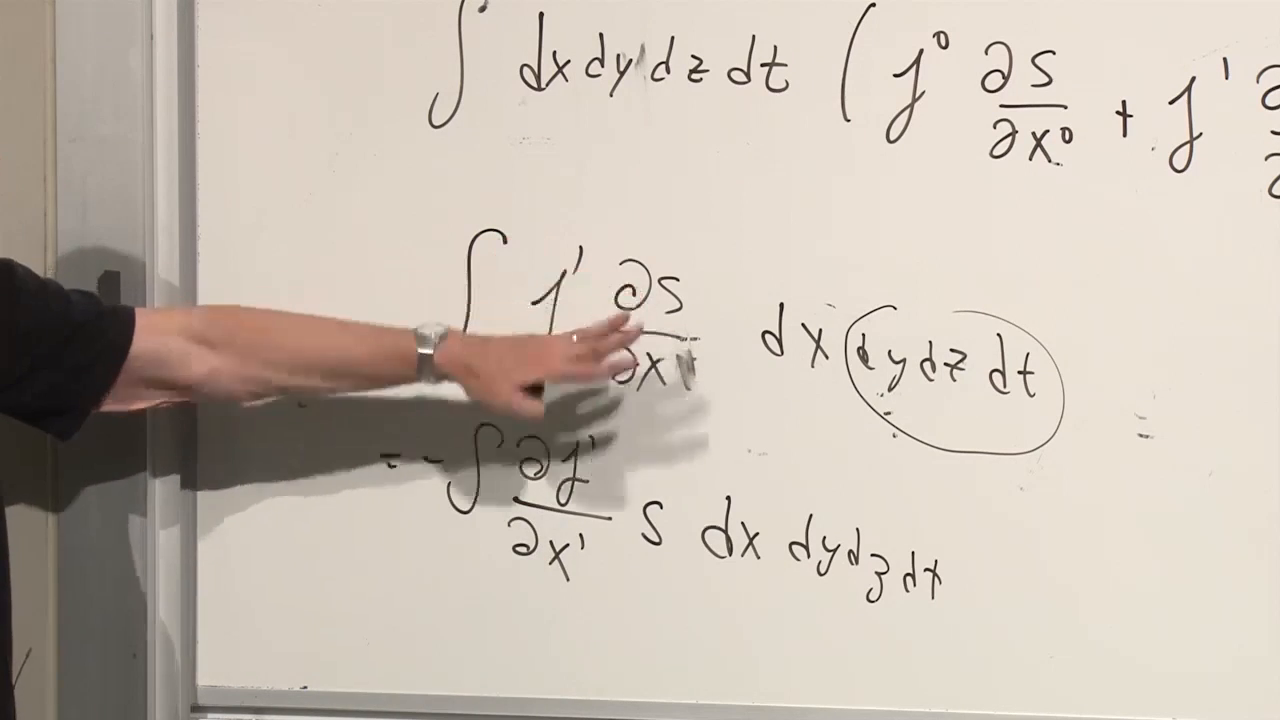
\includegraphics[width=\linewidth]{lecture_09_figure_21.png}
\caption{代表的な部分積分により、微分がゲージ関数から電流へと移される。}
\par\smallskip
\textit{講義フレーム: 01:20:45。}
\end{figure}

四つの成分をすべて集めると
\begin{equation}
\delta_\chi S_{\mathrm{int}}
=
\int d^4x\,\chi\,\partial_\mu J^\mu.
\label{eq:gauge-variation-continuity}
\end{equation}
したがって
\begin{equation}
\partial_\mu J^\mu=0
\quad\Longrightarrow\quad
\delta_\chi S_{\mathrm{int}}=0.
\end{equation}
仮定された境界条件の下では、源の相互作用がゲージ不変であるのは、まさに電流が局所的に保存されているときである。

\begin{classroomqa}
\audiencequestion{
\(\nabla\cdot\mathbf J=0\) のみを要求するだけで十分か。}
\lecturerresponse{いいえ。四つの項すべてが必要である:
\[
\partial_\mu J^\mu
=
\dot\rho+\nabla\cdot\mathbf J=0.
\]
第一の項は固定された箱における電荷密度の変化である。非零の空間的発散は、その変化によって釣り合わされるときには許される。\lecturetimestamp{01:22:00}}
\end{classroomqa}

\section{源のあるマクスウェル方程式}

完全な電磁場のラグランジアン密度は
\begin{equation}
\boxed{
\mathcal L
=
-\frac14F_{\mu\nu}F^{\mu\nu}
-J^\mu A_\mu.
}
\label{eq:full-maxwell-lagrangian}
\end{equation}
である。源の項は \(A_\nu\) の微分を含まないので、\eqref{eq:maxwell-canonical-derivative} を変えず、
\begin{equation}
\frac{\partial\mathcal L}{\partial A_\nu}=-J^\nu.
\end{equation}
に寄与する。したがってオイラー--ラグランジュ方程式は
\begin{equation}
-\partial_\mu F^{\mu\nu}=-J^\nu,
\end{equation}
または
\begin{equation}
\boxed{\partial_\mu F^{\mu\nu}=J^\nu.}
\label{eq:sourced-maxwell-from-action}
\end{equation}
を与える。

\begin{figure}[H]
\centering
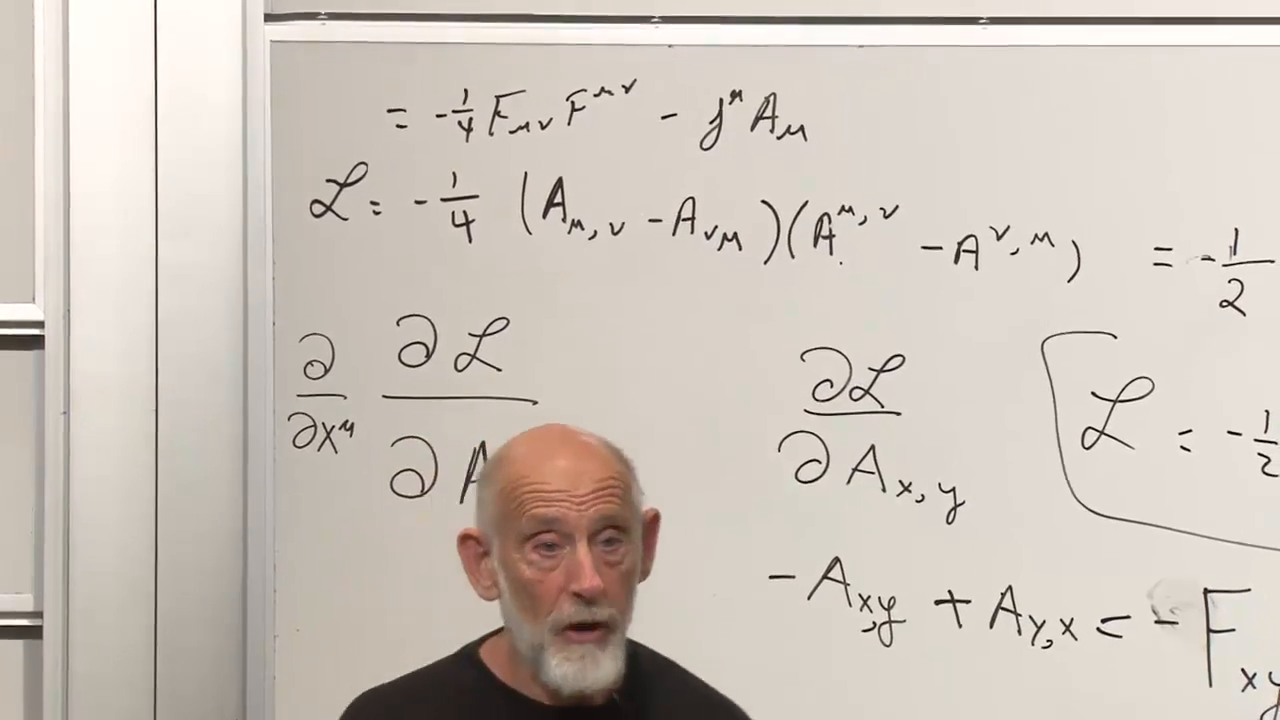
\includegraphics[width=\linewidth]{lecture_09_figure_22.png}
\caption{自由項と源の項を、代表的なオイラー--ラグランジュ微分とともに示したもの。}
\par\smallskip
\textit{講義フレーム: 01:25:00。}
\end{figure}

保存しない与えられた電流は、同時に二つの破綻を引き起こす。相互作用作用はゲージ不変でなくなり、源のあるマクスウェル方程式は無矛盾でなくなる。電荷は、その境界を通る補償的な流束なしに、ある領域の内部で単に消えることはできない。

\section{マクスウェル方程式が保存則を与え返す}

この両立性は場の方程式から直接読み取ることができる。\eqref{eq:sourced-maxwell-from-action} の \(\partial_\nu\) を取ると
\begin{equation}
\partial_\nu J^\nu
=
\partial_\nu\partial_\mu F^{\mu\nu}
=0,
\label{eq:antisymmetry-implies-continuity}
\end{equation}
となる。なぜなら、微分は \(\mu\leftrightarrow\nu\) の下で対称である一方、\(F^{\mu\nu}\) は反対称だからである。

講義ではこれを三ベクトル形式でも確認し、その確認によって生きた符号の誤りが露呈する。ガウスの法則から始める:
\begin{equation}
\rho=\nabla\cdot\mathbf E.
\end{equation}
時間で微分すると:
\begin{equation}
\dot\rho=\nabla\cdot\dot{\mathbf E}.
\label{eq:rho-dot-div-edot}
\end{equation}
暫定的に板書された方程式は
\begin{equation}
\dot{\mathbf E}
=
-\nabla\times\mathbf B+\mathbf J.
\label{eq:provisional-wrong-source-sign}
\end{equation}
と書かれていた。その発散を取ると
\begin{equation}
\dot\rho=\nabla\cdot\mathbf J,
\end{equation}
となる。なぜなら回転の発散は消えるからである。これは \eqref{eq:continuity-vector-l9} と矛盾する。

\begin{figure}[H]
\centering
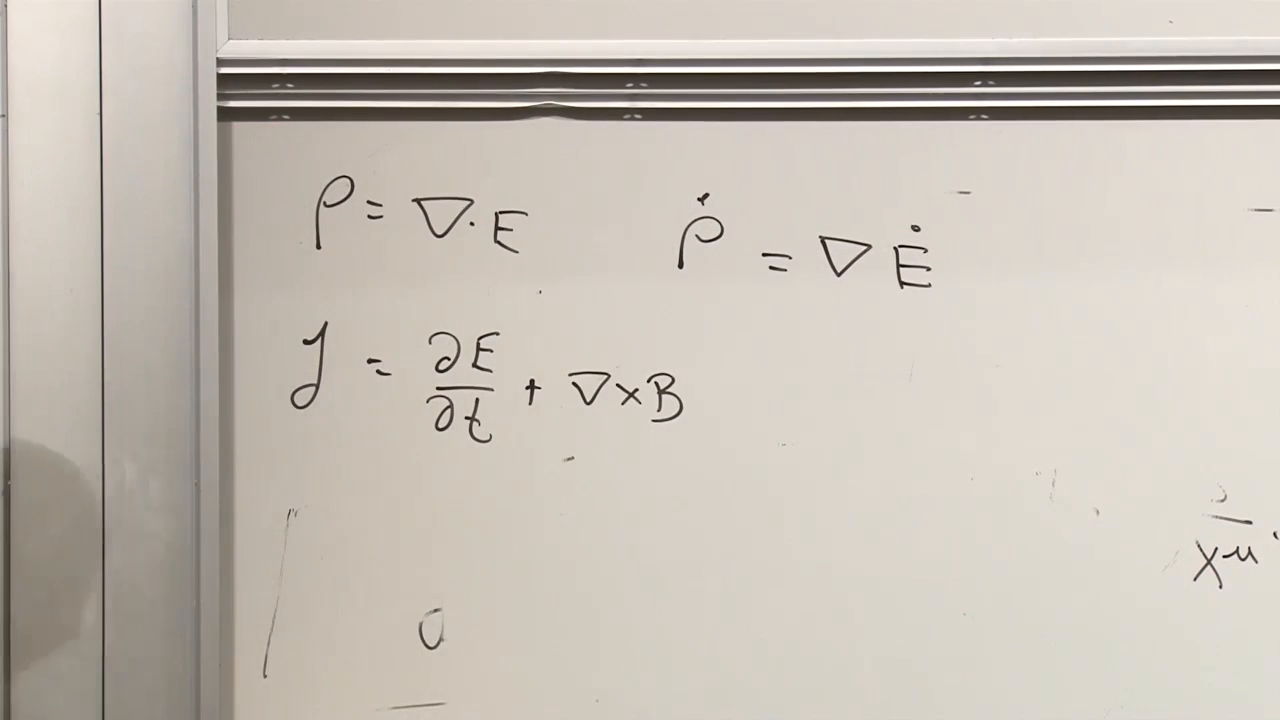
\includegraphics[width=\linewidth]{lecture_09_figure_23.png}
\caption{誤った連続の式の符号を生み出す、暫定的なプラス\(\mathbf J\)の板書方程式。}
\par\smallskip
\textit{講義フレーム: 01:27:00。}
\end{figure}

この不一致は隠されない。計算はその場でたどり直され、要求される連続の式が述べられ、聴衆の一人が方程式を確認して源の符号を特定する。慣習的に無矛盾な成分方程式は
\begin{equation}
\boxed{
\dot{\mathbf E}+\nabla\times\mathbf B=-\,\mathbf J,
}
\label{eq:corrected-source-sign}
\end{equation}
または
\begin{equation}
\dot{\mathbf E}
=
-\nabla\times\mathbf B-\mathbf J.
\end{equation}
である。ここで方程式 \eqref{eq:rho-dot-div-edot} と
\eqref{eq:corrected-source-sign} から
\begin{align}
\dot\rho
&=
\nabla\cdot
\left(-\nabla\times\mathbf B-\mathbf J\right)
\nonumber\\
&=
-\nabla\cdot\mathbf J,
\end{align}
が得られ、これはまさに局所的な電荷の保存である。

\begin{figure}[H]
\centering
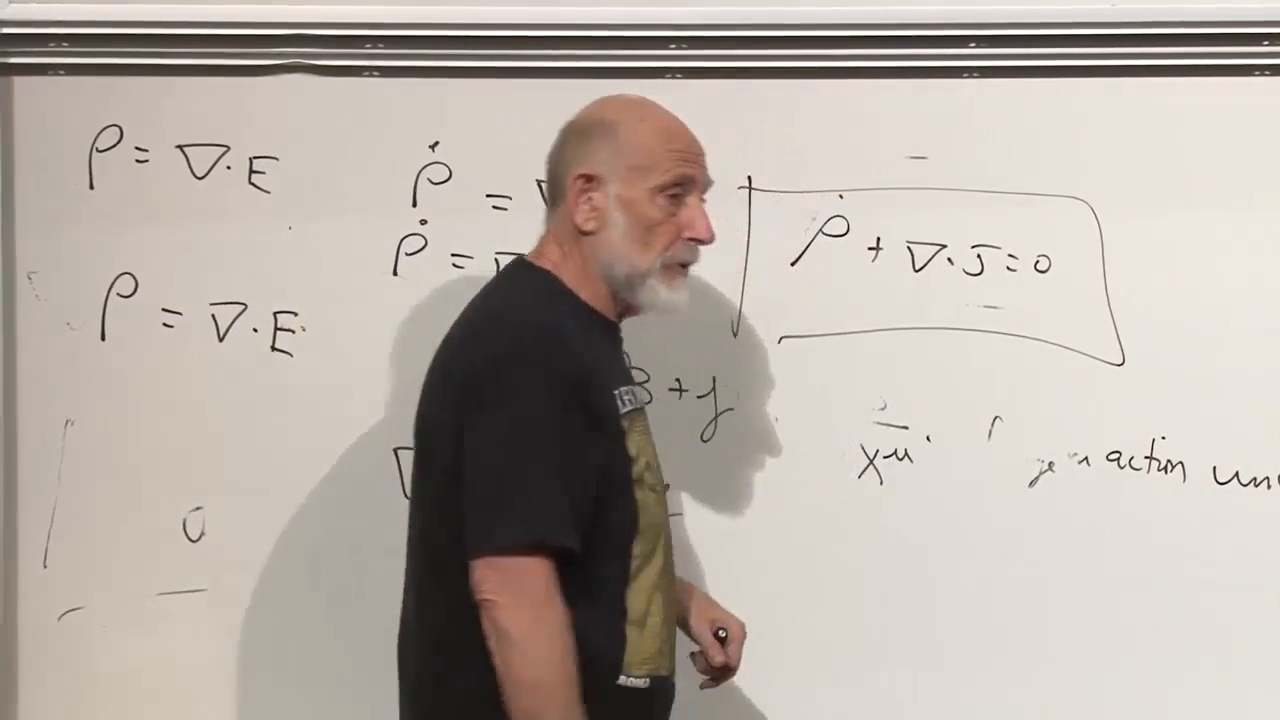
\includegraphics[width=\linewidth]{lecture_09_figure_24.png}
\caption{修正された源の符号と、回復された連続の式。}
\par\smallskip
\textit{講義のフレーム：01：31：00。}
\end{figure}

\begin{classroomqa}
\audiencequestion{右辺の電流項は
\(-\mathbf J\)であるべきか。}
\lecturerresponse{はい。講義全体で用いている場のテンソルの規約では、
\(\partial_\mu F^{\mu\nu}=J^\nu\)の空間部分は
\(\dot{\mathbf E}+\nabla\times\mathbf B=-\mathbf J\)である。
この修正により、発散の計算は
\(\dot\rho+\nabla\cdot\mathbf J=0\)を再現し、先行する
共変な作用の導出を変えることはない。\lecturetimestamp{01:30:17}}
\end{classroomqa}

\section{どちらの原理が基本的か}

\begin{classroomqa}
\audiencequestion{この推論は循環しているのだろうか。我々は電荷保存を用いて作用をゲージ不変にし、次にその作用を用いてマクスウェル方程式を導き、マクスウェル方程式は電荷保存を含意する。}
\lecturerresponse{これらの主張は互いに両立しており、自らの結論を仮定する循環論証ではない。観測されたマクスウェル方程式から出発して連続の式を発見し、次に
\(-J^\mu A_\mu\)がゲージ不変な結合として認識される、としてもよい。あるいは、局所性、ローレンツ不変性、ゲージ不変性、および作用から出発してもよい。ゲージ不変性は保存電流を要求し、作用はマクスウェル方程式を与える。あるいは、電荷が局所的に消滅しないという物理的事実を第一義と見なしてもよい。どの道筋も同じ構造に到達する。\lecturetimestamp{01:31:11}}
\end{classroomqa}

最も経済的な構成的道筋を問うならば、局所性、ローレンツ不変性、ゲージ不変性、およびラグランジアン原理の組み合わせが
\begin{equation}
-\frac14F_{\mu\nu}F^{\mu\nu}-J^\mu A_\mu
\end{equation}
を選び出し、したがってマクスウェルの動力学方程式を選び出す。この三角形の一つの項目をより基本的と呼ぶことは、一部は好みの問題である。重要な事実は、それらの項目が整合していることである。

\section{なぜ\emph{ゲージ}という語なのか}

\begin{classroomqa}
\audiencequestion{数学は明快であるが、ここで
\emph{ゲージ}という語は何を意味するのか。}
\lecturerresponse{この名称は歴史的な時代錯誤である。ゲージは、圧力を基準に対して測る場合のように、選ばれた零点を指すことがある。ヘルマン・ワイルはもともとこの考えを長さの局所的な標準に関連づけたが、その解釈は正しい物理学ではなかった。この自由度が量子波動関数の位相に正しく結びつけられたとき、この用語は生き残った。現在の古典的計算では、
\(A_\mu\)を\(\partial_\mu\chi\)だけ変えても、記述上の零点が変わるだけで
\(F_{\mu\nu}\)は変わらない。より深い量子的な意味は後回しにする。
\lecturetimestamp{01:34:49}}
\end{classroomqa}

歴史的な呼び名は、作用する主張を曖昧にしてはならない。すなわち、\eqref{eq:gauge-transform}で関係づけられるポテンシャルは同じ電磁場を記述する。したがってゲージ自由度はポテンシャル記述の冗長性であり、一方で場のテンソルはゲージ不変である。

\section{なぜ二つのマクスウェル族は非対称に見えるのか}

\begin{classroomqa}
\audiencequestion{電場と磁場がそれほど対称的ならば、なぜ一方のマクスウェル族はビアンキ恒等式として現れ、他方は運動方程式から来るのか。}
\lecturerresponse{源のない電磁気学では、双対ポテンシャルを導入して役割を交換できる。運動方程式であったものがビアンキ恒等式になり、その逆も成り立つ。物理的な非対称性は源を通じて入ってくる。電荷は観測されているが、素粒子の磁気単極子は観測されていない。電荷と磁荷を交換する厳密な通常の対称性があれば、対応するスペクトルをもつ磁気的な相方が期待されるが、それらは見られない。より洗練された理論は依然として磁荷や電気--磁気双対性を含みうるが、それは現在の導出の範囲を超えている。\lecturetimestamp{01:37:11}}
\end{classroomqa}

したがって、源のない方程式は電気--磁気の入れ替え構造をもつが、観測される源の部門は電気的な記述を選ぶ。それは単なる活字上の規約以上のものであるが、自由な平面波に見られる対称性を無効にするものではない。

\section{何が組み立てられたか}

講義を通る道筋はこれで完結した：
\begin{enumerate}
\item マクスウェル方程式は平面波が横波であることを強制し、電場と磁場は直交し、分散関係は
      \(\omega=ck\) となる。
\item ビアンキ方程式はポテンシャルから従う恒等式であり、
      縮約された方程式は動力学方程式である。
\item 局所性とローレンツ不変性は作用密度へと導き、ゲージ不変性は \(A_\mu A^\mu\) を排除し、
      \(F_{\mu\nu}\) から作られるスカラーを選び出す。
\item 自由作用
      \(-\tfrac14F_{\mu\nu}F^{\mu\nu}\) は真空マクスウェル方程式を与える。
\item 相互作用 \(-J^\mu A_\mu\) がゲージ不変であるのは、電流が連続の方程式を満たすとき、まさにそのときに限る。
\item 源を含む作用は
      \(\partial_\mu F^{\mu\nu}=J^\nu\) を与え、反対称性から
      \(\partial_\mu J^\mu=0\) が再び得られる。
\end{enumerate}

これは膨大な構造である。ラグランジュ力学、相対論的場の理論、電気力学、ローレンツ不変性、ゲージ不変性、そして局所的な電荷保存が、一つの議論の部分となった。これを消化する唯一の確実な方法は、方程式からもう一度始め、各導関数と符号を手で追い通すことである。
